% mnras_template.tex 
%
% LaTeX template for creating an MNRAS paper
%
% v3.0 released 14 May 2015
% (version numbers match those of mnras.cls)
%
% Copyright (C) Royal Astronomical Society 2015
% Authors:
% Keith T. Smith (Royal Astronomical Society)

% Change log
%
% v3.0 May 2015
%    Renamed to match the new package name
%    Version number matches mnras.cls
%    A few minor tweaks to wording
% v1.0 September 2013
%    Beta testing only - never publicly released
%    First version: a simple (ish) template for creating an MNRAS paper

%%%%%%%%%%%%%%%%%%%%%%%%%%%%%%%%%%%%%%%%%%%%%%%%%%
% Basic setup. Most papers should leave these options alone.
\documentclass[fleqn,usenatbib]{mnras}

% MNRAS is set in Times font. If you don't have this installed (most LaTeX
% installations will be fine) or prefer the old Computer Modern fonts, comment
% out the following line
\usepackage{newtxtext,newtxmath}
% Depending on your LaTeX fonts installation, you might get better results with one of these:
%\usepackage{mathptmx}
%\usepackage{txfonts}

% Use vector fonts, so it zooms properly in on-screen viewing software
% Don't change these lines unless you know what you are doing
\usepackage[T1]{fontenc}
\usepackage{ae,aecompl}
\usepackage{color}
\newcommand\khb[1]{{\color{magenta}#1}}
\newcommand\edits[1]{{\color{red}#1}}
\newcommand\aab[1]{{\color{green}#1}}

%%%%% AUTHORS - PLACE YOUR OWN PACKAGES HERE %%%%%

% Only include extra packages if you really need them. Common packages are:
\usepackage{graphicx}	% Including figure files
\usepackage{amsmath}	% Advanced maths commands
\usepackage{amssymb}	% Extra maths symbols
\usepackage{textgreek}
\usepackage{enumitem}
%%%%%%%%%%%%%%%%%%%%%%%%%%%%%%%%%%%%%%%%%%%%%%%%%%

%%%%% AUTHORS - PLACE YOUR OWN COMMANDS HERE %%%%%

% Please keep new commands to a minimum, and use \newcommand not \def to avoid
% overwriting existing commands. Example:
%\newcommand{\pcm}{\,cm$^{-2}$}	% per cm-squared

%%%%%%%%%%%%%%%%%%%%%%%%%%%%%%%%%%%%%%%%%%%%%%%%%%

%%%%%%%%%%%%%%%%%%% TITLE PAGE %%%%%%%%%%%%%%%%%%%

% Title of the paper, and the short title which is used in the headers.
% Keep the title short and informative.
\title[Abbie=Smart Person]{Serious Titles are Boring: predicting the future of dark matter halos is fun.}

% The list of authors, and the short list which is used in the headers.
% If you need two or more lines of authors, add an extra line using \newauthor
\author[Very Smart]{
Genius 1,$^{1}$\thanks{E-mail: mn@ras.org.uk (KTS)}
Genius 2,$^{2}$
and Genius 3$^{2,3}$
\\
% List of institutions
$^{1}$Royal Astronomical Society, Burlington House, Piccadilly, London W1J 0BQ, UK\\
$^{2}$Department, Institution, Street Address, City Postal Code, Country\\
$^{3}$Another Department, Different Institution, Street Address, City Postal Code, Country
}

% These dates will be filled out by the publisher
\date{Accepted XXX. Received YYY; in original form ZZZ}

% Enter the current year, for the copyright statements etc.
\pubyear{2018}


% Don't change these lines

\hypersetup{draft} %% ABBIE DELETE THIS LATER THIS IS BAD
\begin{document}
\label{firstpage}
\pagerange{\pageref{firstpage}--\pageref{lastpage}}
\maketitle

% Abstract of the paper
\begin{abstract}
The evolution of a dark matter halo in a dark matter only simulation is governed purely by Newtonian gravity, making a clean testbed to determine what halo properties drive its fate. Using machine learning, we predict the survival, mass loss, final position, and merging time of subhalos within a cosmological N-body simulation, focusing on what instantaneous initial features of the halo, interaction, and environment matter most. Survival is well predicted, with our model achieving 96.5\% accuracy using only 3 parameters from the initial interaction. However, the mass loss, final location, and merging times are much more stochastic processes, with significant margins of error between the true and predicted quantities for much of our sample. The redshift, orbital eccentricity, relative velocity, and the masses of the host and subhalo are the only relevant initial parameters for determining subhalo evolution. In general, subhalos that enter their hosts at a mid-range of redshifts (typically z = .67-.43) are the most challenging to make predictions for, across all of our final outcomes. More circular subhalo orbits are also easier to predict, except for in the case of predicting disruption, where the opposite appears to be true. We conclude that the detailed evolution of individual subhalos within N-body simulations is quite difficult to predict, pointing to a stochasticity in the merging process. We discuss implications for both simulations and observations.
\end{abstract}

% Select between one and six entries from the list of approved keywords.
% Don't make up new ones.
\begin{keywords}
me -- genius -- smart
\end{keywords}

%%%%%%%%%%%%%%%%%%%%%%%%%%%%%%%%%%%%%%%%%%%%%%%%%%

%%%%%%%%%%%%%%%%% BODY OF PAPER %%%%%%%%%%%%%%%%%%

\section{Introduction}

According to the standard \textLambda CDM model of cosmology, dark matter structures in the universe form hierarchically through series of mergers, with larger halos continuously growing through the accretion of smaller subhalos. Once independent halos themselves, these subhalos sink to the center of their "host" halos, losing mass to their hosts along their orbits due to tidal effects and dynamical friction, the effects of which have been studied in detail (\citet{Tormen1998}, \citet{Weinberg1989}, \citet{Bosch1999}, \citet{Hayashi2003}, \citet{Taffoni2003}, \citet{Gan2010}, \citet{VandenBosch2017}). However, as has been shown by modern cosmological N-body simulations, a significant number of such subhalos retain some of their mass, surviving as substructures within their hosts today. The study of these substructures has been fundamental to our understanding of many areas of astrophysics, from large-scale structure (\citet{Knebe2004}, \citet{Zentner2003}) to the formation and evolution of galaxies (\citet{Hayashi2009}, \citet{Kazantzidis2009}, \citet{Simha2016}), which rely on both accurate final subhalo populations and the evolution of these populations within these cosmological simulations (\citet{Diemand2007}, \citet{Giocoli2007}).

Galaxy formation and evolution is commonly studied through modeling the evolution of the subhalos that these galaxies inhabit, with tools such as semi-analytic models (\citet{Taylor2003}, \citet{Zentner2004}, \citet{Penarrubia2005}, \citet{Jiang2016}). These techniques typically rely on merger trees constructed from N-body simulations, along with analytic treatments of the physical processes that cause their evolution. These semi-analytic models often perform quite well, reproducing the statistical properties of subhalo populations. Other works have focused on reproducing specific properties of subhalos, such as disruption rates, mass loss histories, spatial distributions within host halos, and merging timescales. 

Although much work has been done to better model these processes and create prescriptions for subhalo evolution, the reliability of tuning models to the evolution within N-body simulations has remained relatively unexplored. N-body simulations produce consistent subhalo mass functions and the evolution of these populations has been thoroughly studied (\citet{Gao2004}, \citet{Onions2012}, \citet{Jiang2016a}, \citet{Chua2016}) and much recent work has been done to better constrain the low mass end of the subhalo mass function to increase our understanding of smaller satellites (\citet{Munshi2018}). However, it has not been explored in detail whether the evolution of an individual subhalo within these simulations is a truly deterministic process. Models for subhalo evolution that are tuned to the evolution within N-body simulations (\citet{Penarrubia2005}, \citet{Gan2010}, \citet{Hiroshima2018}) reflect the noise and uncertainty in the merging process within the simulation. It may be that subhalo evolution within N-body simulations is somewhat stochastic, such that interactions with similar properties do not necessarily behave in similar ways, adding unforseen complications when using these models.

In this work, we use a merger tree generated from the dark matter only simulation VISHNU, available on the the Theoretical Astrophysical Observatory (\citet{Bernyk2014}), in order to determine the evolution and fate of subhalos, quantified by the aforementioned final quantities (i.e survival/disruption, mass loss, final location within host halo, merging timescale) using machine learning. We model these final conditions from initial conditions at the time of a subhalo entering its host. Using physically-motivated parameters from the time of the subhalos entry, we use machine learning to predict these final quantities of the subhalo, in the hopes of investigating to what degree subhalo fate is motivated by these parameters and to what degree the interaction is stochastic and cannot be predicted. If the mass loss from a subhalo is deterministic, a machine learning algorithm should be able to successfully map subhalo initial conditions to their fates. On the other hand, if there is a level of stochasticity in subhalo fate, there will remain large prediction errors, even when using a complete set of parameters.

Machine learning has emerged as a powerful tool in astrophysics with a variety of applications, such as galaxy classification (\citet{Barchi2019MachineCatalog}, \citet{Nolte2019GalaxyData}), exoplanet detection (\citet{Schanche2018Machine-learningSurveys}), and gravitational wave noise removal (\citet{Cavagli2018FindingLearning}), and has recently been used with cosmological simulations to predict galaxy properties from halo properties (\citet{Kamdar2016}), populate halos with galaxies (\citet{Agarwal2017}), connect initial conditions to final halos (\citet{Lucie-Smith2018}), and predict the halo masses of galaxies (\citet{Calderon2019PredictionApproach}). The ability of machine learning models to approximate any function using a large set of parameters provides a useful means of revealing complicated correlations when a direct analytic function cannot be found. Notably, \citet{Nadler2017} recently used machine learning to predict the survival or disruption of subhalos in a hydrodynamic simulation, using the initial conditions of their counterparts in a dark matter only simulation. They were quite successful, accurately predicting the results of 85\% of their test set of subhalos. Works like this are encouraging that machine learning can be used to fit these complicated interactions. 

In this work, we instead focus on dark matter only simulations, where we predict not only survival, but more quantitative metrics such as the amount of mass loss, the final position, and the duration of the merging time for a subhalo. By using a complete set of physical parameters to make these predictions, we hope to reveal what subhalo parameters are the most closely tied to -- and thus what physical processes most strongly drive -- this evolution. While we expect these additional quantities to be more difficult to predict, even in a dark-matter only simulation with simpler physics, than a binary prediction for disruption, the ability or inability of machine learning models to make predictions in the first place can inform us about the determinism of a model. Predictions that are not successful, despite having this complete parameter set available to them, may point to problems in the assumption that subhalos evolve in a predictable way.

As mentioned, many works have already attempted to either model these subhalo evolution processes from well-understood physics, or investigate trends in subhalo populations within simulations to better understand what drives subhalo evolution. As such, we look to these works to select similar or the same initial parameters that have been found to be important for subhalo evolution to use in our model. The topic of subhalo disruption has a particularly rich body of work. Several works (\citet{Ghigna2000}, \citet{Diemand2004}, \citet{Gao2004}, \citet{Zentner2004}, \citet{Penarrubia2005}, \citet{Diemand2007}) have found that redshift of entry is overwhelmingly important in determining the survivability of subhalos, finding that the majority of surviving subhalos were accreted more recently than z=1. \citet{Gao2004}, \citet{Giocoli2009}, and \citet{Gao2011} find that the abundance of subhalos is lower for host halos of fixed mass that have higher concentrations, but note that higher concentration halos on average form earlier and thus would have less surviving substructure because their substructure is accreted earlier and spends more time orbiting inside the host. \citet{Klimentowski2010} find that many subhalos that are destroyed do not complete even one pericenter passage, but many subhalos that do survive have completed more than one pericenter passage. They also find that surviving subhalos tend to have eccentric orbits. \citet{Diemand2004} find that slower subhalos with low orbital energies were preferentially destroyed, resulting in a positive velocity bias in the subhalo distribution within clusters. \citet{Yang2009} model the fraction of surviving subhalos as a function of the subhalo to host halo mass ratio, with good results. \citet{Tormen1998} find similar results, with larger mass ratios leading to more rapid disruption. \citet{Gill2004} find only weak dependence of the subhalo disruption rate on the mass of the host halo.

As subhalos typically disrupt after losing a significant amount of their mass, we expect many of the parameters that determine subhalo survival to also be of significant importance to subhalo mass loss. Additionally, some works have focused specifically on the topic of subhalo mass loss. \citet{Gao2004} look at populations of subhalos in a wide variety of host halos and find that subhalo mass loss does not strongly depend on the mass of the host halo. \citet{Taylor2003} model subhalo mass loss in a static host potential and find that the eccentricity of the subhalo orbit and the subhalo concentration are the dominant determinants of mass loss, with subhalos losing a significant portion of their mass during each pericenter passage, resulting in more radial orbits losing mass more quickly. \citet{VanDenBosch2005} look at the average mass loss rates of subhalos using only the redshift and subhalo to host halo mass ratio, and find good agreement with subhalo mass functions from simulations. Several additional works (\citet{Taylor2001}, \citet{Hayashi2003}, \citet{Kampakoglou2007}, \citet{Gan2010}, \citet{Han2016}) have modeled subhalo positions and internal structure at each timestep to analytically model their evolution. Although these works give deeper insights to the relative importance of the physical processes at work on these subhalos, our machine learning models do not explicitly model the evolution over time of our subhalos, so the parameters used by those works are less relevant here.

The final distributions of subhalos within their hosts have also been closely studied. \citet{Angulo2009} find that the radial distributions of subhalos does not depend on host halo mass or redshift, but does depend on the suhalo to host halo mass ratio. Similarly, \citet{Nipoti2018} find that subhalos that merge with the central parts of their host halos tend to have larger subhalo to host halo mass ratios than those merging with the outer parts of the host halo, which may suggest that mass ratio can help predict the final location of a subhalo. \citet{Reed2005} find a trend of decreasing subhalo spin closer to the host center, suggesting that lower spin halos may have more success surviving to z=0 when orbiting at small fractions of the host radius. If this is due to higher spin subhalos being more susceptible to tidal stripping, this trend could also be important for our other predicted quantities. 

Analytic predictions of merging timescales for subhalos have been found by a number of previous works. \citet{Wetzel2010} fit a function to determine the time until satellite removal after accretion using only the subhalo to host halo mass ratio. \citet{Boylan-Kolchin2007} and \citet{Jiang2007} perform similar studies, modeling the effects of dynamical friction to determine galaxy merging timescales, using the subhalo to host halo mass ratio, the circularity and energy of the subhalo orbit, and the virial radius of the host halo, and the dynamical time at the host halo's virial radius. \citet{McCavana2012} model merging timescales using similar parameters. Although they find different dependencies on these parameters than \citet{Boylan-Kolchin2007} or \citet{Jiang2007}, the parameters dominating the merging timescale remain the same.

In Section \ref{sec:simulation}, we describe the simulation and data that we use, as well as the methods we employ to properly reduce the data into our desired sample. In Section \ref{sec:ML Methods}, we cover the machine learning methods we use to create our predictive models. In Section \ref{sec:feature selection}, we discuss the feature selection methods we use to gain intuition and decide on which parameters are the most important for each model to make predictions. In Section \ref{sec:Results}, we share the results of our models for predicting each of our outcomes, including their performance and which parameters were needed as inputs to the model. Finally, in Section \ref{sec:Conclusion} we discuss implications of our results for both observation and theory.

\section{Description of the Data}
\label{sec:simulation}
\begin{figure}
	% To include a figure from a file named example.*
	% Allowable file formats are eps or ps if compiling using latex
	% or pdf, png, jpg if compiling using pdflatex
	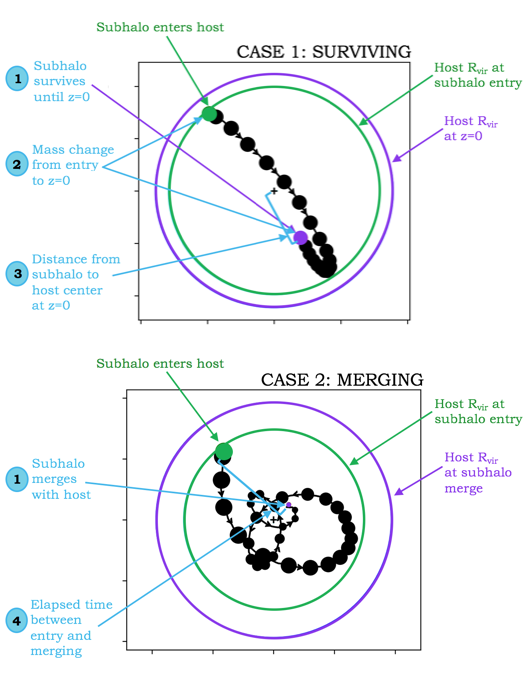
\includegraphics[width=\columnwidth]{Figures/explanatory_figures}
	\vspace{-15pt}
    \caption{An example of a surviving (top) and merging (bottom) interaction between a subhalo and host halo. The orbit of these two subhalos are shown within the radius of their respective host halos, shown by the larger, unfilled circles. Point size corresponds to subhalo mass along the orbit, plotted at each eighth timestep. The green point and circle show initial quantities, at the timestep right before the subhalo enters its host. The orange point and circle show final quantities, at either the timestep right before the subhalo dissolves in the merging case, or at the final timestep in the simulation in the surviving case. Predicted quantities (gold) are labeled and numbered in the order we will present them throughout the paper.}
    \label{fig:explanatory_figures}
\end{figure}

Our analysis makes use of VISHNU, a cosmological N-body simulation with 1000 snapshots for exquisite time resolution; no snapshot is separated by more than 3.2 $\times$ 10\textsuperscript{7} years. VISHNU contains 1680\textsuperscript{3} particles in a volume of 130h\textsuperscript{-1} cMpc and uses WMAP-1 cosmology (\citet{Spergel2003}); $\Omega$\textsubscript{m} = 0.25, $\Omega$\textsubscript{$\Lambda$} = 0.75, $\Omega$\textsubscript{b} = 0.04, $\sigma$\textsubscript{8} = 0.8, \textit{n\textsubscript{s}} = 1.0, \textit{h} = 0.7). Each dark matter particle has mass \textit{m\textsubscript{p}} = 3.215 $\times$ 10\textsuperscript{7}h\textsuperscript{-1} M\textsubscript{\(\odot\)}, and the force resolution is \edits{\textbf{INSERT NUMBER} (2.2 kpc?)} parsecs. The ROCKSTAR halo finder was used to identify halos and subhalos (\citet{Behroozi2013}), and merger trees were constructed with Consistent-Trees (\citet{Behroozi2013a}).

Starting with halos at \textit{z}=0, we use the merger trees to identify the most massive progenitors of all host halos within the simulation, and track the subhalos within. These subhalos are allowed to have further substructure inside of them but cannot, at any point during their infall, become sub-substructure themselves. To help mitigate resolution uncertainties, we select only subhalos with a minimum of 1000 particles (total mass 3.215 $\times$ 10\textsuperscript{10}h\textsuperscript{-1} M\textsubscript{\(\odot\)}) at their time of accretion. We define the accretion time as the last timestep before a subhalo enters its host. This mass cut reduces our sample from 1284058 subhalos to 121343 subhalos.

Once it has been accreted, the subhalo must have one of two fates: merge with the host, or remain a bound, identified subhalo within that host until today. We define the point of merging as the point right before dissolution of the subhalo, the last timestep in the simulation where it is identified as its own entity. Following uncertainties in subhalo mass loss shown by \citet{Bosch2018}, once a subhalo has lost more than 90\% of its mass, we also consider it to be merged. This cut changes the fates of 21929 subhalos, around 18\% of our total sample, but ensures a more consistent definition of merging that is less sensitive to resolution errors.
    
Figure \ref{fig:explanatory_figures} shows examples of the orbits of the two types of interactions that we consider. In the top panel, we show an example of a surviving interaction, where the subhalo orbits for some time, losing mass but not dissolving before z=0. In the bottom panel, we show an example of a merging interaction, where the subhalo orbits and loses mass until reaching the center of the host and dissolving at some time before z=0. The four quantities that we will predict are shown in blue and numbered by the order that they will be presented in Section \ref{sec:Results}. We predict the survival of both the surviving and merging populations as one complete sample. When we predict the mass loss and final position quantities, we do so for only our surviving population. When we predict the merging time quantity, we do so for only the merging population. 

In addition to making cuts for resolution, some interactions were removed due to their unphysical behavior, likely as a result of errors in the merger tree generation or halo finding. 1474 subhalos were removed that more than tripled their mass during infall. These subhalos were likely misidentified as they moved close to the center of the host, instead being assigned the mass of another subhalo or the host itself. 327 subhalos were removed because their initial mass was larger than that of their supposed hosts. Altogether, we culled about an additional 1.5\% of the total sample with these cuts.

%Although we have attempted to correct for these errors, there remains the possibility that erroneous cases still exist within our sample. We have made a hard cut to remove halos that gain mass, but there may be still be cases where an identification of a halo was changed within our sample. Additionally, some orbits are known to look strange or have instantaneous mass loss or gain that can be harder to properly check for. \textit{Some discussion of the cases that could possibly still exist in the data due to difficulty in being able to filter them out/ find a general way to search for them? Lots of things that double/half mass in a step and then look semi-regular again. Should I mention that? Something that gives some estimation of how many cases might be like this? To ensure that it's not some large part of the sample and the reason we can't predict things. Mention that we removed about 2\% of the total number so even if you assume the same portion is wrong it shouldn't be the source of the stochasticity?}

\begin{figure*}
	% To include a figure from a file named example.*
	% Allowable file formats are eps or ps if compiling using latex
	% or pdf, png, jpg if compiling using pdflatex
	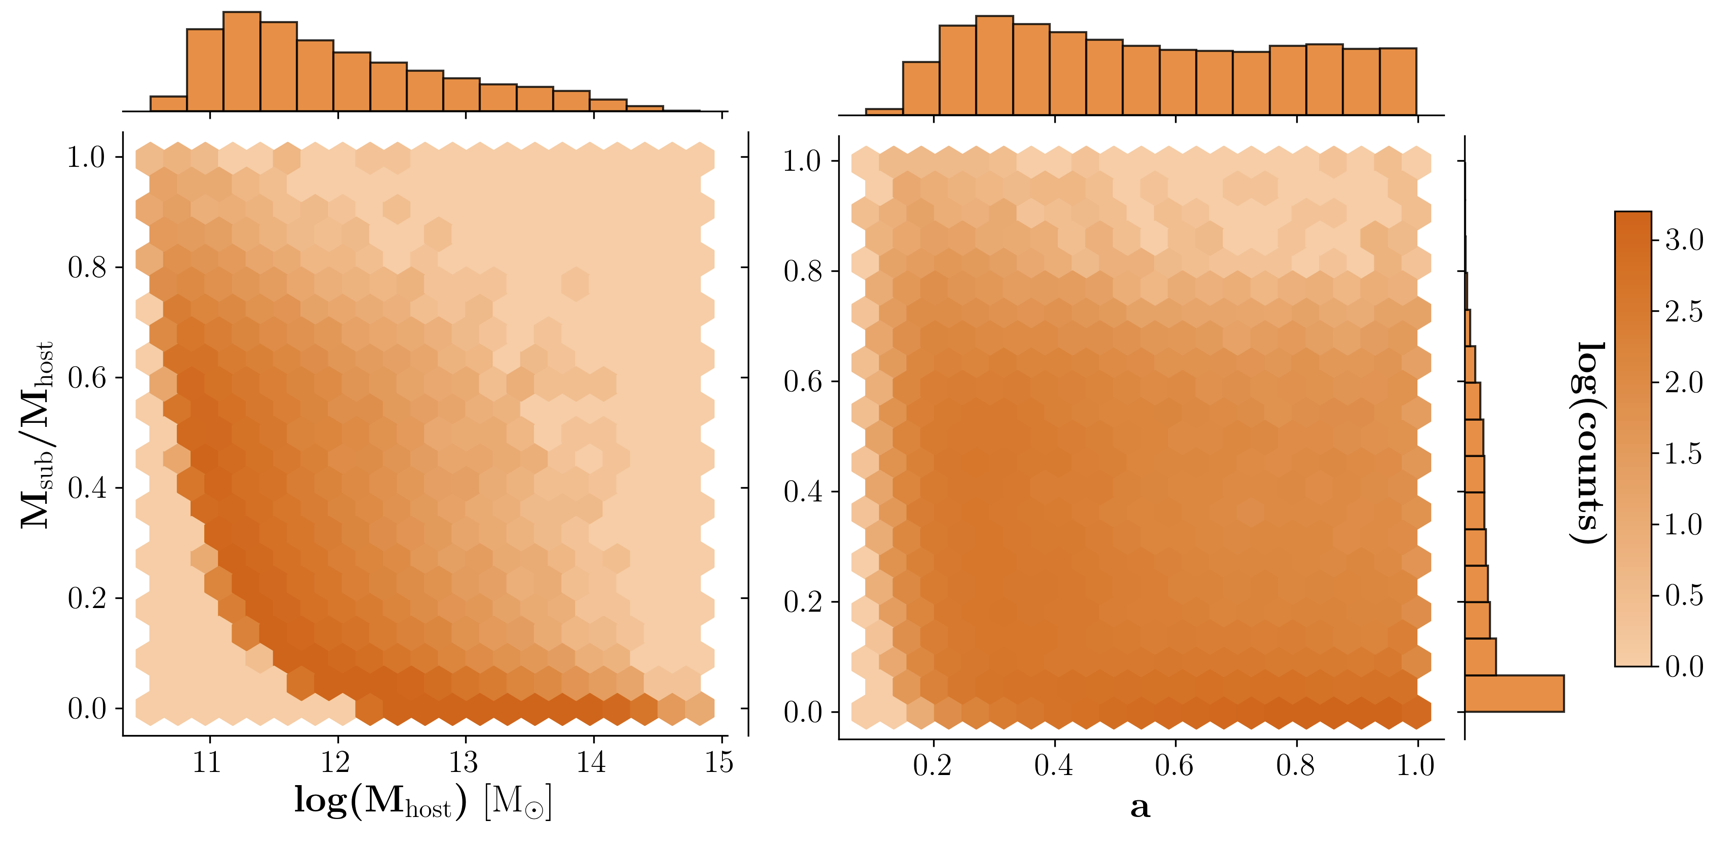
\includegraphics[width=\textwidth]{Figures/combined_distributions_logbin}
	\vspace{-20pt}
    \caption{Distributions of the merging interactions within our sample, in two different two-dimensional spaces. The left panel shows the distribution of interactions in the space of the host mass (x-axis) and the mass ratio (y-axis) of the interaction. The right panel shows the distribution of mergers in the space of the scale of initial entry of the subhalo (x-axis) and again, the mass ratio of the interaction on the y-axis. Within each hexagonal bin, the counts of interactions are shown, on a logarithm scale, by the colorbar. Histograms show the one-dimensional distribution of host masses (above the left panel), scale of entry (above the right panel) and mass ratios to the right of the right panel). Most interactions occur at lower mass ratios and for smaller host halos, but the spaces are still well-spanned over a range of interactions in both panels. The chosen cut of 1000 particles (M = 3.215 $\times$ 10\textsuperscript{10}h\textsuperscript{-1} M\textsubscript{\(\odot\)}) for subhalos upon entry is clearly shown in the left panel. Imposing this cut and requiring that host halos be larger than their subhalos means that, for very small host halos, the only subhalos within our dataset are those with masses more similar to their hosts. Additionally, it imposes that none of our host halos have masses below 3.215 $\times$ 10\textsuperscript{10}h\textsuperscript{-1} M\textsubscript{\(\odot\)} as well.}
    \label{fig:combined_distributions_logBin}
\end{figure*}

    Our resulting sample includes a total of 119543 subhalo-halo interactions, with 76442 of such being mergers and 43101 being survivors. Distributions of this sample with respect to host masses, mass ratios, and the scale factor of the time of entry are shown in Figure~\ref{fig:combined_distributions_logBin}. The most common interactions in our sample are mergers of unequal masses that occurred more recently. However, our sample also spans the space of more equal mass and higher redshift mergers, with hundreds of interactions shown in many of the bins in Figure~\ref{fig:combined_distributions_logBin}. The effects of our chosen particle cut can also be clearly seen in Figure~\ref{fig:combined_distributions_logBin}. Because subhalos must have 1000 particles at their time of entry, this results in a minimum initial mass of 3.215 $\times$ 10\textsuperscript{10}h\textsuperscript{-1} M\textsubscript{\(\odot\)} for both the subhalo and host halo, given that a host halo must also be at least as large as its subhalo. In the left panel of Figure~\ref{fig:combined_distributions_logBin}, this results in an area of no data with low mass hosts and unequal masses, because most subhalos of low mass hosts are too low mass to be included in our sample.
\par
    For both the host halo and subhalo at the timestep of infall, and at either the timestep right before merging or at z=0, we take several physically-motivated parameters to describe the interaction between the halos. We also calculate a few additional parameters that were not given explicitly from Consistent-Trees merger trees. We divide our final set of initial parameters, which were used as input parameters to the machine learning models to make predictions, into four main categories. Internal halo parameters are those that are properties of the individual halos themselves. These parameters do not depend on the other halo in the interaction, instead giving important information about the structure of the halos as individuals. Relative halo parameters describe properties of the halos that are dependent on either other halos within the simulation or the simulation itself. Orbital parameters provide information about the initial trajectory of the subhalo's infall path. Environmental parameters describe the influence of larger scale environment around the subhalo and its host. In total, this gives us 26 input parameters, with definitions:
    
\vskip 0.1in
    \noindent\textbf{Internal Halo Parameters:}
    \begin{itemize}[leftmargin=.4cm,topsep=0pt]
        \item \textbf{M\textsubscript{sub}}: M\textsubscript{200b} of the subhalo. This is defined using a spherical overdensity, including only those particles that were assigned to the subhalo. Because M\textsubscript{200b} is defined using the background mass density of the universe, this definition is not affected by pseudo-evolution.
        \item \textbf{M\textsubscript{host}}: M\textsubscript{200b} of the host halo. This is defined using a spherical overdensity, including all particles that are assigned as being part of the host halo. Therefore, this mass definition also includes the mass of all subhalos within the host.
        \item \textbf{R\textsubscript{sub}}: R\textsubscript{200b} of the subhalo.
        \item \textbf{R\textsubscript{host}}: R\textsubscript{200b} of the host halo.
        \item \textbf{c\textsubscript{sub}}: the concentration of the subhalo, defined as R\textsubscript{200b}/R\textsubscript{s}, where R\textsubscript{s} is the scale radius of the subhalo.
        \item \textbf{c\textsubscript{host}}: the concentration of the subhalo, defined as R\textsubscript{200b}/R\textsubscript{s}, where R\textsubscript{s} is the scale radius of the host halo.
        \item \textbf{\textlambda\textsubscript{sub}}: Bullock spin parameter of the subhalo, defined as in \citet{Bullock2001}.
        \item \textbf{\textlambda\textsubscript{host}}: Bullock spin parameter of the host halo, defined as in \citet{Bullock2001}.
        \item \textbf{T\textsubscript{sub}}: the triaxiality parameter of the subhalo. Calculated from the definition given in \citet{Franx1991}:
        \begin{equation}
            T = \frac{1 - (b/a)^2}{1 - (c/a)^2}
        \end{equation}
        where b/a is the minor/major axis ratio and c/a is the intermediate/major axis ratio.
        \item \textbf{T\textsubscript{host}}:  the triaxiality parameter of the host halo, calculated as above.
    \end{itemize}
\vskip 0.1in
    \noindent\textbf{Relative Halo Parameters:}
    \begin{itemize} [leftmargin=.4cm,topsep=0pt]
        \item \textbf{a}: the scale factor of the universe.
        \item \textbf{M\textsubscript{ratio}}: the ratio of subhalo to host halo masses.
         \item \textbf{max(M\textsubscript{subs,sub})}: M\textsubscript{200b} of the most massive sub-subhalo within the subhalo. 0 if subhalo has no sub-substrucutre. 
        \item \textbf{max(M\textsubscript{subs,host})}: M\textsubscript{200b} of the most massive subhalo already within the host halo at the time of the selected subhalo's entry. Does not include the selected subhalo. 0 if no other subhalos are present.
        \item \textbf{N\textsubscript{subs,sub}}: the total number of sub-subhalos within the subhalo.
        \item \textbf{N\textsubscript{subs,host}}:  the total number of subhalos within the host halo. Does not include the selected subhalo.
    \end{itemize}
\vskip 0.1in
    \noindent\textbf{Orbital Parameters:}
    \begin{itemize} [leftmargin=.4cm,topsep=0pt]
        \item \textbf{d\textsubscript{rel}}: relative absolute distance between the centers of the subhalo and host halo.
        \item \textbf{v\textsubscript{rel}}: relative total velocity between subhalo and host halo, calculated in the reference frame of the subhalo.
        \item \boldmath$\epsilon$\unboldmath: eccentricity of subhalos initial orbit. Calculated as described in \citet{Wetzel2011}:
        \begin{equation}
            \epsilon = \sqrt{1 + \frac{2EL^2}{(GM\textsubscript{host}M\textsubscript{sub})^2\mu}}
        \end{equation}
        In this definition, $\epsilon$ = 1 is a perfectly elliptical orbit, and orbits that are initially unbound have eccentricities greater than 1.
        \item \boldmath$\theta$\unboldmath: inclination of subhalos initial orbit. Calculated as $L_\textsubscript{total}/L_\textsubscript{max}$, the ratio between the total angular momentum of the subhalo orbit and the angular momentum of an orbit with the same velocity magnitude and orbital distance, but with the entire velocity component in the direction perpendicular to the direction of the host center. In this definition, $\theta$ = 1 is a perfectly radial inclination.
    \end{itemize}
\vskip 0.1in    
    \noindent\textbf{Environmental Parameters:}
    \begin{itemize}[leftmargin=.4cm,topsep=0pt]
        \item \textbf{F\textsubscript{tid, 1Mpc}}: The tidal force on the subhalo, due to all surrounding halos out to 1 Mpc from the subhalo center, that are not the host halo.
        \item \textbf{F\textsubscript{tid, 2Mpc}}: The tidal force on the subhalo, due to all surrounding halos out to 2 Mpc from the subhalo center, that are not the host halo.
        \item \textbf{F\textsubscript{tid, 4Mpc}}:
        The tidal force on the subhalo, due to all surrounding halos out to 4 Mpc from the subhalo center, that are not the host halo.
        \item \boldmath$\rho$\unboldmath\textbf{\textsubscript{1Mpc}}: The density of the surrounding sphere with radius 1 Mpc from the subhalo center.
        \item \boldmath$\rho$\unboldmath\textbf{\textsubscript{2Mpc}}: The density of the surrounding sphere with radius 2 Mpc from the subhalo center.
        \item \boldmath$\rho$\unboldmath\textbf{\textsubscript{4Mpc}}: The density of the surrounding sphere with radius 4 Mpc from the subhalo center.
    \end{itemize}
\vskip 0.1in  
Parameters that are taken at the end of the interaction, either at the time the subhalo dissolves or at z=0, are used to define the quantities that the machine learning models will predict. These parameters include:
%\renewcommand{\theenumi}{\arabic{enumi}}
    \begin{enumerate}[leftmargin=.4cm]
        \item [1.] \textbf{survival}: a 0 or 1, depending on if the subhalo exists above the required mass threshold at z=0 (survives, 1) or if the subhalo has either merged with its host or fallen below the mass threshold at some time before z=0 (merges, 0). Predicted for all subhalos.
        \item [2.] \textbf{M\textsubscript{sub,f}}: the M\textsubscript{200\textsubscript{b}} of the subhalo at the end of the interaction. Only predicted for subhalos that survive until z=0.
        \item [3.] \textbf{d\textsubscript{rel,f}}: relative absolute total distance between subhalo and host halo centers at the end of the interaction, normalized by the virial radius of the host halo. Only predicted for subhalos that survive until z=0.
        \item [4.] \textbf{t\textsubscript{merge}}: the elapsed time between accretion of a subhalo into the host radius and the time of merging with the host. Only predicted for subhalos that dissolve at some time before z=0.
    \end{enumerate}
\par
    As preparation for using machine learning, we split the data into \textit{train}  and \textit{test} sets, with 80\% of the data for training and 20\% to test. These subsamples are selected randomly from the total sample. The data are scaled and normalized to be distributed as a Gaussian with zero mean and unit variance, meaning that before giving each parameter (X) to the model, we transform it by: 
    \begin{equation}
        X\textsubscript{norm} = \frac{X - \mu}{\sigma}
    \end{equation} 
    using \texttt{StandardScaler} from the \texttt{scikit-learn preprocessing} package, where \textmu{} is the mean of the unscaled data and \textsigma{} is the standard deviation. This scaling is necessary for many machine learning models, as large variations in parameter ranges can affect model accuracy.
    Each time we train our machine learning models, we further divide the training set into training and validation sets, also using an 80\%/20\% split. From the original dataset, this means that 20\% of our data is used only for final testing, while 80\% of our data set is repeatedly divided into training and validation sets. The use of these validation sets allows us to tune model hyperparameters while leaving the testing set untouched to ensure that it cannot be overfit.

\section{Machine Learning Methods}
\label{sec:ML Methods}
The machine learning algorithms we use in this work come from the \texttt{scikit-learn} package for python. Subhalo survival is a classification problem, so we use a random forest algorithm. On the other hand, predictions of the amount of mass loss, the final position, and merging time are all classic regression problems, so we use the gradient boosting regressor algorithm. Although we refer the reader to the \texttt{scikit-learn} documentation for a full description of these algorithms, we briefly describe these methods, and others that we tried, below.

\subsection{Random Forests}
\label{sec:rf}
Random forest classifiers use a compilation of decision trees to reach consensus on a prediction. These decision trees repeatedly split the data on the values of its input parameters, binning the data into small subsets until bins are small enough that they generally give the correct output. In a random forest, many individual decision trees are trained on random subsets of the full dataset. Because random forests are a type of bagging - or bootstrap aggregating - method, the classification for an object is then the majority vote of all of the trees. This means that the trees that make up the ensemble are individual from each other - each tree makes an independent prediction for the classification of an object in the testing set.

There are several hyperparameters of the algorithm that we tune in order to get the best-fitting model. The \textit{n\_estimators} hyperparameter sets the number of estimators, in this case decision trees, that will be separately trained and used in the final consensus. Using too few decision trees removes the power of using multiple trees. In general, using too many trees is not a concern, as the performance of random forests is not decreased by adding large numbers of trees. For much larger datasets, adding too many trees can lead to much longer training times. However, given our relatively small number of samples, this isn't much of a concern in our training.  The \textit{max\_depth} hyperparameter sets the maximum number of decisions that can be made in each tree before reaching a classification decision. Effectively, this sets the maximum number of input parameters each decision can use, as at each depth level of a decision tree, an input can only follow one path, splitting on one parameter. The \textit{max\_leaf\_nodes} hyperparameter sets the maximum number of new nodes a parameter can be divided into from a single leaf, which is one single path that a decision has taken at a given depth level. We note that, if this value is too small, the decision tree may need to split on the same input parameter at multiple depth levels. We keep other parameters of the algorithm set to their default values, which can be found in the \texttt{scikit-learn} documentation. In general, these other hyperparameters tend to allow the user to fine-tune the criterion for the decision tree to make a split, or add criterion to prevent overfitting, both of which we did not find necessary when creating our model.

One of the main advantages of random forest algorithms are that they are less prone to overfitting, especially compared to a single decision tree. Because each decision tree is given a subset of the data and considers a random group of parameters, the consensus of all decision trees is more robust to unseen data. This is important especially in cases like this work, where we have a large number of training examples to determine a small number of phenomena. Random forests are also useful in their ability to deal with correlations between input parameters, another important feature given the strong correlations between many of our parameters. Unfortunately, the results of a random forest are much less straightforward to interpret than that of single decision trees. Because each decision tree only uses a portion of the information, some of the decision trees within the forest may be very poor predictors. While this makes it impossible to extract a single decision path for a given input, it allows for a robust extraction of the most prominent features, which the \texttt{scikit-learn} random forest classifier ranks in a function called \texttt{feature\_importances\_}. This function rates the importance of training features given their frequency of selection and proximity to the top of the decision trees within the forest. However, strong correlations between features can make this ranking difficult to straightforwardly interpret as well, which we discuss in more detail in Section \ref{sec:feature selection}.

Subhalo survival is particularly amenable to binary classification; we assign 0 to a subhalo for dissolving before z=0, and a value of 1 for surviving until z=0. We train the model using all initial features described in Section \ref{sec:simulation}. Because our set of parameters has strong correlations among several parameters, we do not use the aforementioned order of feature importance given by \texttt{scikit-learn} to inform us about which of our input parameters are most important for making predictions, and instead we use a feature selection method outlined in Section \ref{sec:feature selection} below. We use this order to train models, using the same hyperparameters, on increasingly smaller subsets of the features to confirm the minimum number of features needed to make accurate predictions, and for presentation purposes in our figures.

\subsection{Gradient Boosting Regressors}
\label{sec:gbr} % used for referring to this section from elsewhere
Gradient boosting regressors, like random forests, rely on an ensemble of decision trees to make predictions. However, unlike random forests, gradient boosting regressors rely on boosting methods, meaning that newly trained decision trees are dependent on the results of all the trees trained before them. Models that rely on boosting methods are created in an additive fashion, where new trees are fit to the errors of the current ensemble, then added to the ensemble such that the prediction for any given input is the additive result of all trees. These errors are computed every time before a new tree is trained, as the residual between the current prediction of the model and the true value. The goal of each newly trained tree is to learn the errors of the current model. Then, when adding that tree to the model, the goal is to move the prediction closer to the true value, by appropriately adding or subtracting the amount by which the prediction was wrong.

As with the random forest classifier, several hyperparameters can be tuned to create the best model. The learning rate hyperparameter gives weight to the prediction of each added tree to the ensemble. So, a large learning rate means that the contribution of new trees is very significant, while a smaller learning rate means that the contributions of new trees are weighted to be small. Too small of a learning rate may significantly increase the number of trees that need to be added to the model. However, too large of a learning rate may mean that the corrections of the new trees always overshoot the true value. As with the random forest classifier algorithm, we also tune the \textit{n\_estimators} hyperparameter to determine the number of decision trees to add to the model, and the \textit{max\_depth} and \textit{max\_leaf\_nodes} hyperparamters for individual trees in the gradient boosting algorithm. Other parameters of the algorithm are kept as their default values, which can be found in the \texttt{scikit-learn} documentation.

The advantage of using a gradient boosting regressor is again the reduction of overfitting. Because gradient boosting regressors are ensembles of weak learners, which are easily overfit, giving each weak learner a random subset of the data means the overall ensemble is much less prone to overfitting. This is particularly important given the smaller scope of our regression problem, which uses relatively few parameters for the number of examples in our sample. Additionally, because we expect that only a small subset of our parameters will be important in making these predictions, a model that is able to avoid selecting unimportant parameters is favorable. As with the random forest classifier, the gradient boosting regressor class in \texttt{scikit-learn} also contains a function to report relative feature importances. However, interpreting these results again presents difficulties due to strong correlations between parameters.

For each of our regression problems, we use a gradient boosting regressor to predict the final quantity. A different gradient boosting regression model is created and separately tuned for each of our outcomes we predict. Each model is given all initial features to train on. As with the survival classification problem, due to the difficulty of interpreting the reported feature importances of the algorithm, we use our custom algorithm, outlined in Section \ref{sec:feature selection} to determine the order and relative importance of features for predicting each of our desired quantities. In Section \ref{sec:Results}, we talk in more detail about training the model for each individual final outcome.

\subsection{Other Models}
\label{sec:other models} % used for referring to this section from elsewhere
Although we have chosen to use a random forest classifier and gradient boosting regression for our analysis, several other popular machine learning algorithms would also be well suited to these problems and able to perform similarly. In particular, neural networks have become increasingly popular for a wide variety of applications, for both classification and regression problems, due to their ability to fit to data incredibly well. Several other, arguably more intuitive machine learning algorithms could also be used. The K-nearest-neighbors algorithm, for example, assigns predictions based on the properties of objects in the training set that are similar to the testing object trying to be predicted. To ensure that our model was as well fit and possible without being too overfit, we tried several of such machine learning algorithms before settling on our choices.

In particular, neural networks, random forests, and gradient boosting regressors performed quite similarly, reaching the same maximum accuracy with similar amounts of overfitting for all of our predictors. As such, we chose to use random forests and gradient boosting regressors over neural networks because they are simpler, both in terms of tuning the model and in interpreting its results. We also tried K-nearest-neighbors and support vector machine algorithms, without any accuracy improvement over the aforementioned algorithms for any of our predicted quantities, and worse results for some of our predicted quantities. Because random forests and gradient boosting regressors reached maximum accuracy for all of our quantities, we decided to use only these two algorithms.

\section{Feature Selection}
\label{sec:feature selection} % used for referring to this section from elsewhere
To train our models, we have selected 26 initial parameters (or features) to describe each subhalo/host halo interaction. These parameters are selected to encompass information about the orbit, environment, and individual properties of both the host and subhalo. Although we begin with this large set of parameters for thoroughness, we expect that not all of them will be important for predicting our desired quantities. In order to determine which parameters most strongly affect the predicted quantities, we use a feature selection method. The goal of this feature selection is to select four parameters from the complete set, for each predicted quantity, which are responsible for the most variation in that quantity. Because our set of parameters has strong correlations between several values, we also aim to use a feature selection method that will minimize correlations in the selected subset of features. Although we call the methods described below "feature selection", we emphasize that we do not remove any parameters using these methods. Instead, we will use the order of selected features to determine the order in which we will add features to our models and for display purposes in our figures. During training, all models will still have the opportunity to use all of our parameters, to ensure that no information is missed.

% Best-spaces figure
\begin{figure*}
	% To include a figure from a file named example.*
	% Allowable file formats are eps or ps if compiling using latex
	% or pdf, png, jpg if compiling using pdflatex
	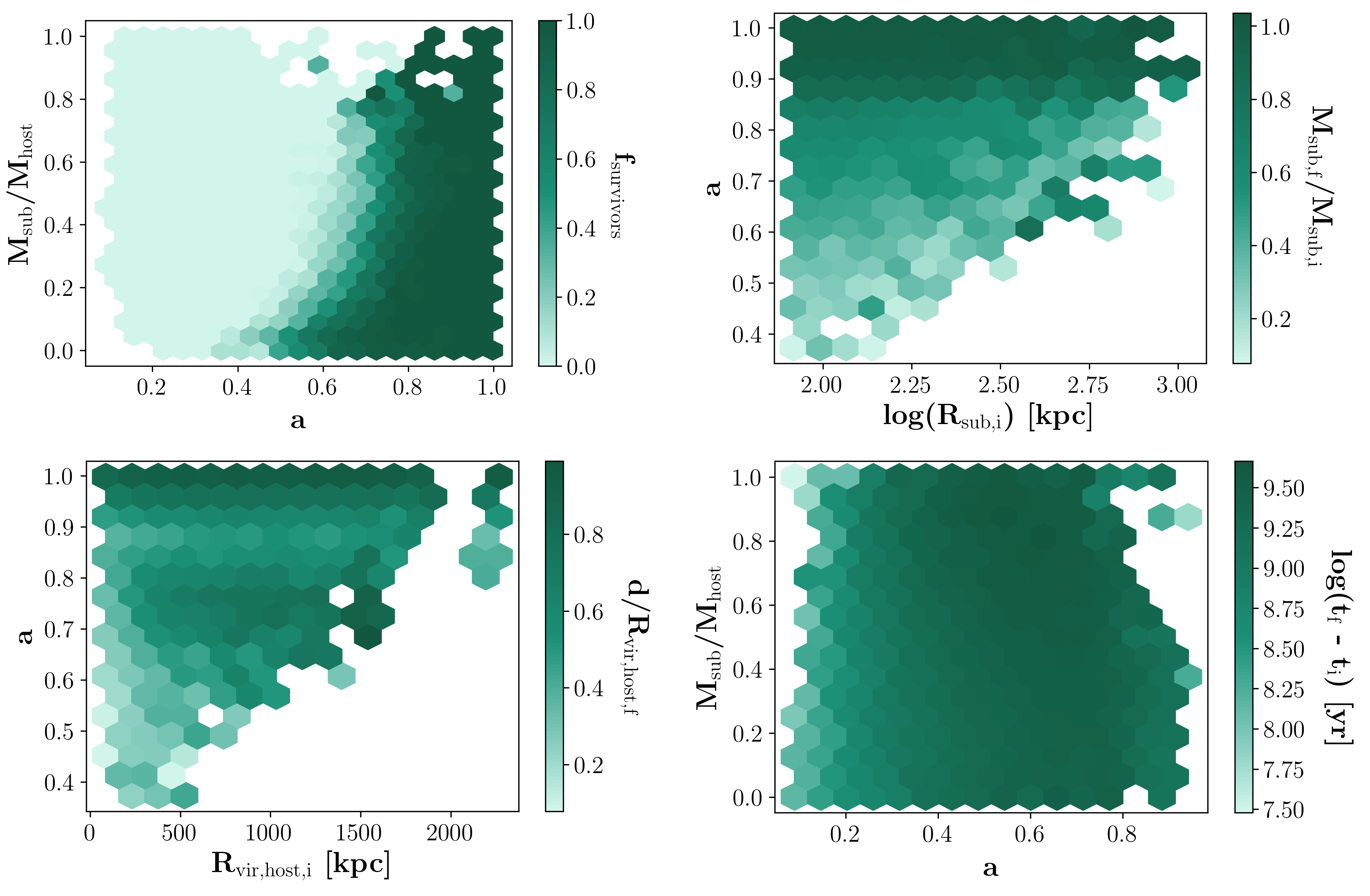
\includegraphics[width=\textwidth]{Figures/bestSpaces}
	\vspace{-15pt}
    \caption{Distributions of the predicted quantity of interest with respect to the two parameters that are most responsible for its variations. In each panel, the parameter that causes the most variation is shown on the x-axis, and the parameter that causes the second most variation is shown on the y-axis. In addition, in each panel the colorbar shows the average values of the quantity of interest within a bin. The top left panel shows the fraction of surviving subhalos. The top right panel shows the fraction of subhalo mass that remains for surviving subhalos. The bottom left panel shows the fractional distance of surviving subhalos from their host's center. The bottom right panel shows the elapsed time for a subhalo to merge. In each instance, some pattern of color striation can be seen to represent the importance of the two parameters shown. However, it is clear that the survival of a subhalo is by far the most drastically divided and well-defined by this two-dimensional space. }
    \label{fig:bestSpaces}
\end{figure*}

We describe the feature selection method using the example case where we wish to predict the final mass of surviving subhalos. We begin by repeatedly binning our desired quantity by each of our feature parameters and checking the variance of the quantity within those bins. For example, we generate bins of the orbital eccentricity, then calculate the average mass loss of subhalos that are within each bin. We then calculate the difference between the lowest and highest values of mean mass loss among the bins, as a measure of the strength of the correlation between final mass and eccentricity. We repeat this process for each of our other feature parameters, and designate the feature that displays the largest such difference as the most important feature. In the next step, we create two-dimensional bins of both this feature and every other feature, and check the average mass loss within two-dimensional bins and determine which second dimension causes the most variance. This allows us to calculate the degree of correlation between mass loss and each remaining feature while controlling for the feature we already selected as most important. The feature that causes the most variance in the mass loss when added as a second dimension is then our second most important feature. We continue with this process, going on to create three-dimensional bins with two features held constant and then four-dimensional bins with three features held constant, until we have extracted four features. After four features, the sample size does not permit further binning of the data in five dimensions, as the bins become too small and noisy to accurately determine a trend. The order of feature importance for each final quantity is then the order in which the parameters were selected using this method.

We find this method useful for two main reasons. First, due to the strong correlations between several of our parameters, it is difficult to interpret feature importance results from the \texttt{scikit-learn} algorithms. This is because the \texttt{scikit-learn} random forest and gradient boosting regressor algorithms calculate feature importance as the information provided by a node, weighted by the fraction of total samples that pass through that node, averaged over all decision trees. This means that two parameters that contain near identical information may have similar importance rankings, despite only one being needed to make accurate predictions, as they take turns being seeded highly in different trees, after which the other one isn't needed anymore. This can also decrease the overall importance ranking of both parameters, because it will make the same parameter be found highly important in some trees, and not important at all in others. We found that ordering parameters according to the \texttt{scikit-learn} functionality did not lead to the quickest information gain when training models with additional parameters. Additionally, because random forests and gradient boosting regressors are built using series of decision trees, the intuition behind those algorithms and these feature selection methods are similar. When building decision trees, features that are ranked higher in the tree are both the most important features, and those that cause the most variance in the final quantity. So, ordering our parameters by the amount of variance they are responsible, while binning to remove correlations with other parameters, leads to a feature order that appears to add information the most quickly.

The results of the four most important features for each of the predicted quantities are shown in Table \ref{tab:FS_table}. The number next to each parameter represents the strength of variance due to that feature. This number is the difference between the maximum and minimum averages of the quantity within bins of that parameter and those ranked higher. In order to make these numbers more easily comparable, we collapse our desired quantities to be between 0 and 1, so a variance of 1 would be the most possible variance and a variance of 0 would be no variance within the bin. For survival, this did not mean changing the quantity at all. For mass loss, final position, and merge time, we normalize the quantities we predict by subtracting the minimum value of that quantity, and dividing by the range of values. For mass loss, we additionally use the log of the masses to collapse them to a less drastic scale. 

Table \ref{tab:FS_table} shows that some parameters, such as the initial scale factor of entry and the inclination of the subhalos orbit, appear as important for all of the predicted quantities. In particular, the initial scale is either the first or second most important parameter for predicting all of our final quantities. These results are already encouraging, as many of these selected features are those that we might expect to be necessary for determining our final quantities. For example, the scale factor at which a subhalo enters the host is intuitively important for all of the quantities, as the amount of time a subhalo spends within its host halo tells us how long it has spent being affected by its host halo, losing mass and falling more to the center. Similarly, we could expect that information such as the subhalo to host halo mass ratio, which informs the strength of dynamical friction, or the orbital inclination, which informs how close the subhalo will get to the center of its host, would also be imperative for determining the fate of a subhalo.

We can already tell, from the relative variance associated with these top four parameters, that some of our predicted quantities may need more than four parameters to make accurate predictions, while others may be able to reach maximum accuracy with fewer parameters. For example, in the case of mass loss, the variance due to the fourth parameter, d\textsubscript{rel}, is small and close to noise. (/edits{Should I say what random noise is somewhere? Variance due to a rando number: .033 for survival, .01 for mass, .02 for position, .024 for time at the 4th depth in the varaition tree.} When comparing this variance to the variance due to a random parameter, the values are similar, suggesting that this fourth parameter may not be needed. On the other hand, in the case of survival and merge time, the fourth parameter, c\textsubscript{sub}, still shows high variance compared to that of a random parameter, suggesting more parameters might provide more information and help our predictions, even though we do not have enough data to bin in the space of a fifth parameter. Although our number of samples limits our ability to probe deeper than four parameters, it does not have the same effect on the machine learning. That is, for our machine learning methods, the number of samples we have is more than sufficient to train the model, so any extra parameters that are needed to make these predictions should emerge when creating our machine learning models. 

Using this ranking of most important features, we look at the values of our predicted quantities within the two-dimensional space of the two parameters most responsible for variations in the outcome. This is shown in Figure \ref{fig:bestSpaces}. For example, the top left panel shows the mean survival fraction, in bins of both initial scale and subhalo to host halo mass ratio. From this figure, we can see how strongly the predicted quantities rely on their chosen features. For survival, the two-dimensional space is clearly divided, suggesting that the survival of a subhalo is already well-determined by only two parameters. For the other quantities, this gradient is less defined, suggesting that either more parameters are needed to make good predictions, or the process is stochastic enough that general trends with respect to our input parameters are harder to find. In particular, the panel for merge time (lower right) in Figure \ref{fig:combined_distributions_logBin} shows little variation in outcome across the entire space of initial scale and subhalo to host halo mass ratio, despite the merging time having the strongest trend of variation with those parameters. From these two-dimensional spaces, we can already see that some of these final quantities, such as survival, may be much more straightforward to predict than others, such as merge time.

% Feature Selection Table
\begin{table}
	\centering
	\caption{The ranking order of most important features for predicting each of the desired quantities. Values next to the chosen feature represent the normalized maximum variation from binning within that parameter, where higher values indicate the parameter is more strongly responsible for changes in the prediction outcome.}
	\label{tab:FS_table}
	\begin{tabular}{c|cccc} % four columns, alignment for each
		\hline
		rank & Survival & Mass Loss & Position & Merge Time\\
		\hline
		1st & a (.997) & R\textsubscript{sub} (.243) & a (.538) & a (.283)\\
		2nd & M\textsubscript{ratio} (.254) & a (.132) & M\textsubscript{ratio} (.214) & M\textsubscript{ratio} (.127)\\
		3rd & $\theta$ (.145) & $\theta$ (.047) &  $\theta$ (.177) & $\theta$ (.091)\\
		4th & v\textsubscript{rel} (.093) & M\textsubscript{host} (.042) & v\textsubscript{rel} (.153) & v\textsubscript{rel} (.058)\\
		\hline
	\end{tabular}
\end{table}

\begin{figure}
	% To include a figure from a file named example.*
	% Allowable file formats are eps or ps if compiling using latex
	% or pdf, png, jpg if compiling using pdflatex
	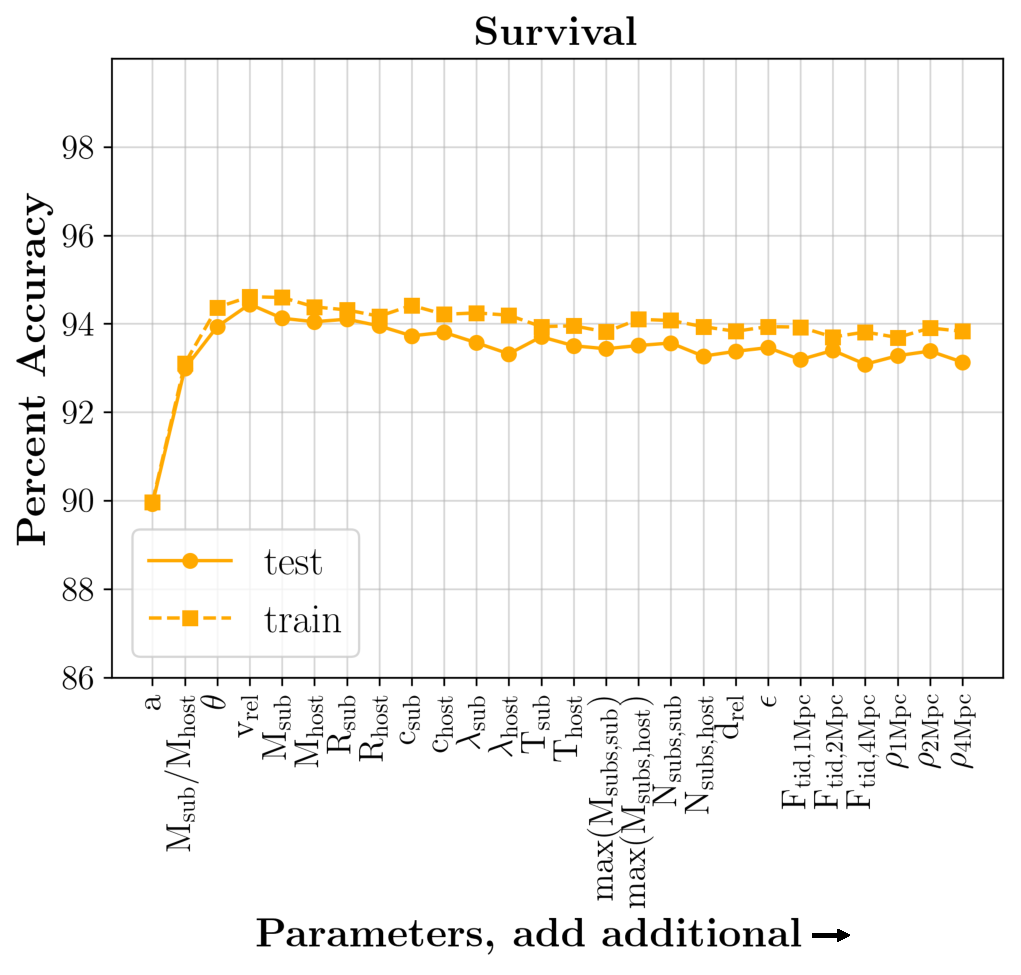
\includegraphics[width=\columnwidth]{Figures/survival_predictions}
	\vspace{-15pt}
    \caption{Accuracy of model's predictions, for both the training and testing sets, when predicting survival. Percentage of the subhalo sample that is predicted accurately is shown on the y-axis. On the x-axis, the parameters used to train the model are shown. For each point, the model was trained using all parameters to the left of that point on the y-axis. The solid line shows the accuracy on the test set, while the dashed line shows the accuracy on the set the model was trained on.}
    \label{fig:survival_predictions}
\end{figure}

\begin{figure}
	% To include a figure from a file named example.*
	% Allowable file formats are eps or ps if compiling using latex
	% or pdf, png, jpg if compiling using pdflatex
	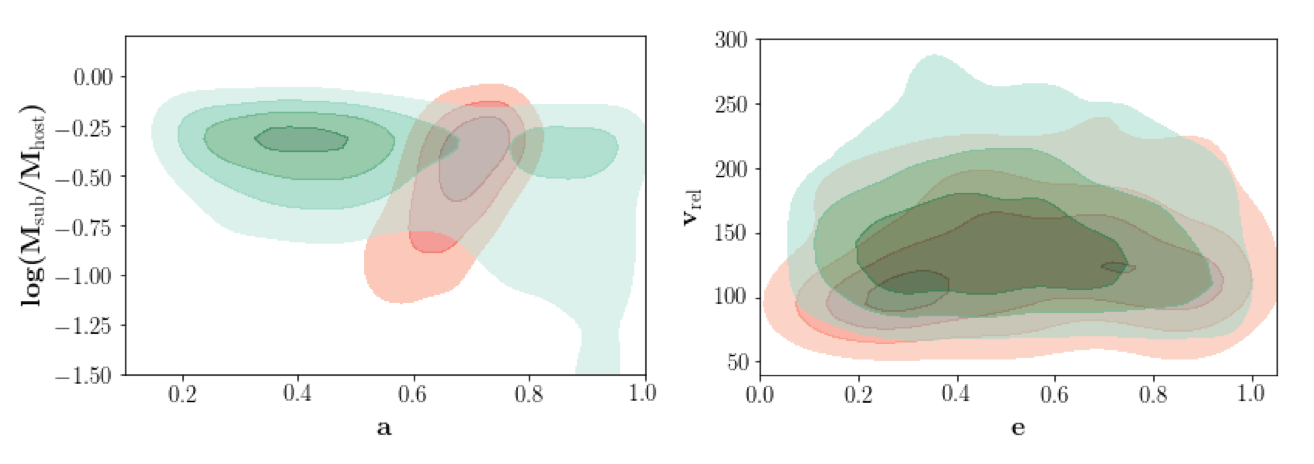
\includegraphics[width=\columnwidth]{Figures/survival_contours}
	\vspace{-20pt}
    \caption{Contours of the accurately and inaccurately predicted subhalos, in two-dimensional spaces of the four most important features. Blue contours show the correctly predicted subhalos, and red contours show the incorrectly predicted subhalos. Contours are divided into 5 sections, with 20\% of subhalos lying within the inner most contour, 40\% lying within the second innermost contour, and so on. The outermost contour is not shaded as to more clearly show the contour regions.}
    \label{fig:survival_contours}
\end{figure}

\section{Results}
\label{sec:Results}
For each of the final quantities, we train a machine learning algorithm, using all available parameters, to predict the outcome value. For each of quantity, we select hyperparameters for the model by repeatedly training iterations of the model using the training set, and checking its accuracy on the validation set, until the best fit with lowest overfitting is achieved. We begin this process by using \texttt{scikit-learn}'s \texttt{GridSearchCV} function, which accepts arrays of values for the desired hyperparameters to be tuned, then repeatedly trains the model on all combinations of the hyperparameters and evaluates each combination's performance. This function includes a \texttt{best\_params\_} attribute, which will return the combination of hyperparameters that leads to the best performance. We then, by inspection, fine-tune the hyperparameters within small ranges around this set. For example, we may begin with a depth hyperparameter of 5 for our model, then check if either raising the depth to 6 or lowering it to 4 with other hyperparameters held constant will give us improvement. We repeat this process for all hyperparameters, until we find a model that achieves high accuracy on both the training and validation sets, indicating that the model is well fit to the data, but with the smallest differences between training and validation accuracy, indicating that the model is minimally overfit. We take this extra step of tuning the hyperparameters by hand because our metrics for accuracy are different than that of the \texttt{score} method that the \texttt{GradientBoostingRegressor} class returns, which \texttt{GridSearchCV} uses to determine the best set of hyperparameters. Fine-tuning these hyperparameters by hand allows us to ensure that each model is optimized for each of our specific accuracy metrics.

Once we have found a set of hyperparameters that performs well without overfitting, we fix this as our model for the given final quantity. Then, we train this model using increasing subsets of our feature parameters and test its performance on our testing set. We begin by adding the four most important parameters, in order of their found importance, from our feature selection methods. Additional feature parameters are then randomly added, until the model is trained with all of our parameters. This gives us an accuracy for our model given not only our complete set of features, but smaller subsets of our features that utilize only the features we found to be important. In this way, we can determine the minimum subset of parameters needed to achieve maximum accuracy. 


In the following subsections, we detail the results of these models, as well as our metrics for determining the accuracy of our predictions in the case of each predicted final quantity. In Section~\ref{sec:survival}, this is discussed in detail for predicting the survival quantity. In Section~\ref{sec:mass loss}, we discuss this in detail for the mass loss quantity. In Section~\ref{sec:position} we discuss the final position quantity, and in Section~\ref{sec:merge time} we discuss the merging time quantity.

\subsection{Survival}
\label{sec:survival} % used for referring to this section from elsewhere

For the entire sample of subhaloes, we first try to predict whether or not a halo will survive until z=0 (assigned a value of 1) or merge with the host sometime before z=0 (assigned a value of 0) by using a random forest classifier. We tune the hyperparameters of this model and find the best results given 50 estimators and a \textit{maximum depth} of 7. We keep the \textit{max\_leaf\_nodes} hyperparameter set to the default (\texttt{None}), allowing an unlimited number of nodes at each depth. The accuracy metric we use to determine the performance of this model is a straightforward categorical accuracy, which is given as the percentage of halos correctly classified as either 0 or 1.

Figure \ref{fig:survival_predictions} shows the accuracy of this model, when trained using increasingly large subsets of our feature parameters. In this figure, each point shows the training or testing accuracy of a model trained with all parameters up to that point on the x-axis. We emphasize that, although we add parameters to the model in an ordered way, the \texttt{scikit-learn} random forest does not use the ordering of input parameters when training a model, and each new subset of parameters requires re-training of the model with that subset. Thus, if the ordering of our parameter additions had been completely random rather than chosen from our feature selection methods, the maximum model accuracy would not change, although the appearance of information gain in Figure \ref{fig:survival_predictions} would. 

As is clearly shown in Figure \ref{fig:survival_predictions}, after the addition of our four most important parameters, a maximum in the accuracy of both the testing and training sets is reached, with an accuracy of 94.6\% on the training set, and 94.4\% on the testing set. The gap between these accuracies is small, suggesting low overfitting. The decrease in accuracy when adding additional paramters beyond these four suggests a lack of information gained by adding any parameter thereafter. Any small increases or decreases in the accuracy beyond the first four parameters are within noise. Additionally, because the model is free at any iteration to use as many of the provided parameters as needed, the maximum accuracy being reached after the addition of only these four parameters suggests that they are the only parameters are necessary to predict the survival of a subhalo. Although the training set generally does better than the test set, the accuracy difference is small and expected due to a small amount of overfitting. The accuracy of the training and testing sets does decrease gradually with the addition of more parameters rather than plateauing. This is likely due to the nature of random forests, where splits within the trees are chosen using a random subset of features. As the number of features with little to no information begins to largely outweigh the number of parameters that do carry information, it becomes more likely to get splits in the trees that are unhelpful to making predictions. We also note that this decrease in accuracy is small (<1\%), so this effect is very minimal.

The four parameters that are needed to achieve this maximum accuracy are: the initial scale of subhalo entry, the ratio of subhalo to host halo mass, the inclination of the subhalo orbit, and the incoming velocity of the subhalo. The initial scale of the subhalo entry is overwhelmingly the most important of these parameters - 90\% of our test sample is accuracy predicted with this parameter alone. With the addition of each of the remaining parameters, a 2.7\%, 1.2\%, and .27\% accuracy percentage is gained for each parameter added, respectively. Within the parameter spaces of these four top parameters, we show in Figure \ref{fig:survival_contours} where the accurately and inaccurately predicted subhalos within our test set lie. There is a clear tendency for subhalos with a\textsubscript{i} =  .6 - .7 to be the most difficult to predict. This agrees with the upper left plot of Figure \ref{fig:bestSpaces}, where a clear division between always surviving and always merging occurs at this value. The shape of this contour also agrees with what we see in Figure \ref{fig:bestSpaces}, where the division of always merging an always surviving subhalos shifts to lower initial scales for smaller subhalo to host halo mass ratios. We note that, although most of the poorly predicted halos exist in this small section of parameter space, 80\% of halos with a\textsubscript{i} =  .6 - .7 are still accurately predicted, significantly better than random guessing. The right panel of Figure \ref{fig:survival_contours} also shows that the innermost contour of the inaccurately predicted subhalos centers around $\texttheta$ = .4, while the innermost contour of the accurately predicted subhalos centers around $\texttheta$ = .8. Although the location of these innermost contours are clearly separated, the total span of eccentricity values is roughly the same. Similarly, the span of values for the subhalo-to-host-halo mass ratio and initial relative velocity are not noticeably very different for the two populations.

To determine if there are significant differences between the correctly and incorrectly predicted subhalos with respect to our additional parameters, we perform a KS test between these distributions, with respect to each of the additional parameters beyond our set of the most important four. In order to ensure that we do not find differences in these distributions due to correlations with our four most important parameters, we find a narrow bin within these four parameters that removes all differences between correctly and incorrectly predicted halos with respect to those four parameters. Then, we perform a KS test between the two distributions within that narrow bin, with respect to all additional parameters. In doing so, we find that the two distributions have a detection above 3\textsigma to be the same, for all of our additional parameters, suggesting that there is no significant difference in any of the additional parameters between correctly and incorrectly predicted subhalos.

\begin{figure}
	% To include a figure from a file named example.*
	% Allowable file formats are eps or ps if compiling using latex
	% or pdf, png, jpg if compiling using pdflatex
	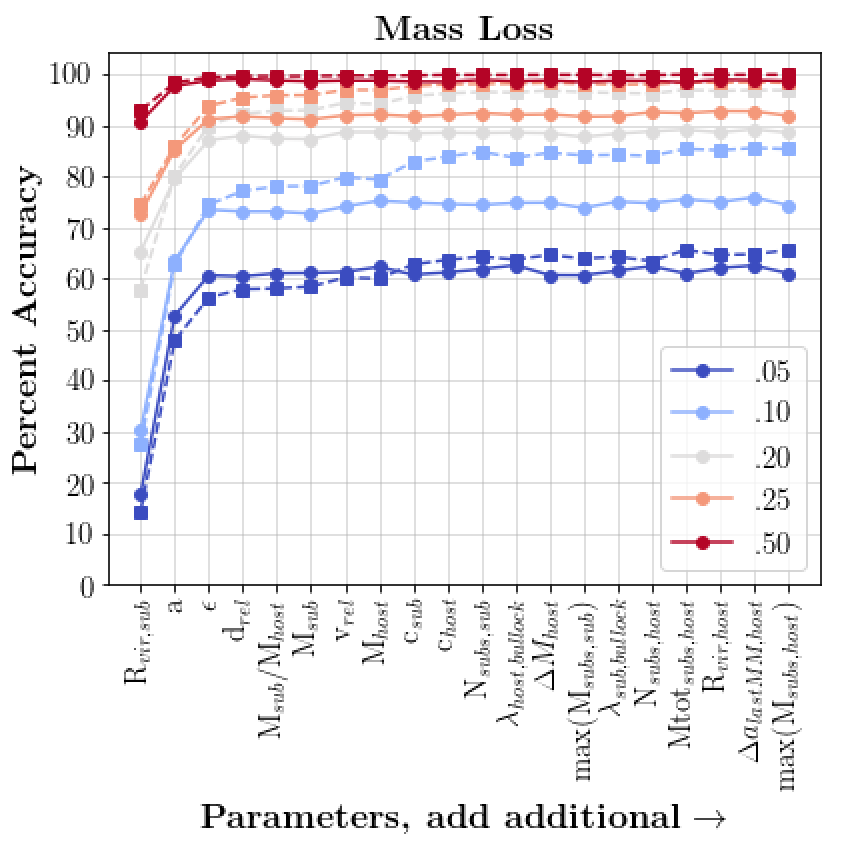
\includegraphics[width=\columnwidth]{Figures/massloss_predictions}
	\vspace{-15pt}
    \caption{Accuracy of model's predictions, for both the training and testing sets, when predicting mass loss. Percentage of accurate predictions is shown on the y-axis. The x-axis shows parameters used to train the model. For each point, the model was trained using all parameters to the left of that point on the y-axis. The solid line shows the accuracy on the test set, while the dashed line shows the accuracy on the set the model was trained on. Different colored lines show the different tolerance values used to define accuracy, as defined in Equation \ref{eq:mass loss}. For a complete description of this accuracy metric, see text.}
    \label{fig:massloss_predictions}
\end{figure}

\subsection{Mass Loss}
\label{sec:mass loss}
For only subhalos that survive until z=0 without being disrupted, we predict the mass of the subhalo at z=0 using a gradient boosting regressor. We tune the hyperparameters of this model and find the best results given 600 estimators, a learning rate of .07, and a \textit{max\_depth} of 3. We keep the \textit{max\_leaf\_nodes} hyperparameter set to the default (None), allowing an unlimited number of nodes at each depth. To determine the accuracy of the model, we define an accuracy metric, using the the difference between true and predicted fractional remaining mass. A subhalo is considered to be accurately predicted if:
\begin{equation}
    \label{eq:mass loss}
    \frac{|M_\textsubscript{pred,f} - M_\textsubscript{true,f}|}{M_\textsubscript{true,i}} - \frac{2m\textsubscript{p}\sqrt{N\textsubscript{p,true,i}}}{M_\textsubscript{true,i}} \leq tol
\end{equation}
Where \textit{tol} is some tolerance value which determines what difference in fractional mass loss is acceptable as accurate. We refer to the quantity given on the left hand side of the equation as the accuracy score for a given subhalo. We then vary the tolerance which we compare this score to, determining what percentage of subhalos are within certain tolerance thresholds. 

The first term in this equation is our primary measurement of the difference between our true and predicted masses. Although the quantity that our machine learning model predicts is the mass of the subhalo, we check accuracy by normalizing this value to the initial mass of the subhalo and comparing true and predicted fractions of initial mass. We do this as to have a metric that equally penalizes errors in prediction for all subhalos, rather than allowing more leniency depending on the subhalo mass. The second term in the equation acts as an additional tolerance to account for poisson noise in the number of particles assigned to the subhalo, which even a perfect predictor of the underlying mass loss process would not reasonably have errors less than. This term is significantly smaller than the first term and only makes a difference in the case of small subhalos, where a small number of particles is a larger portion of the mass than in larger subhalos.

\begin{figure}
	% To include a figure from a file named example.*
	% Allowable file formats are eps or ps if compiling using latex
	% or pdf, png, jpg if compiling using pdflatex
	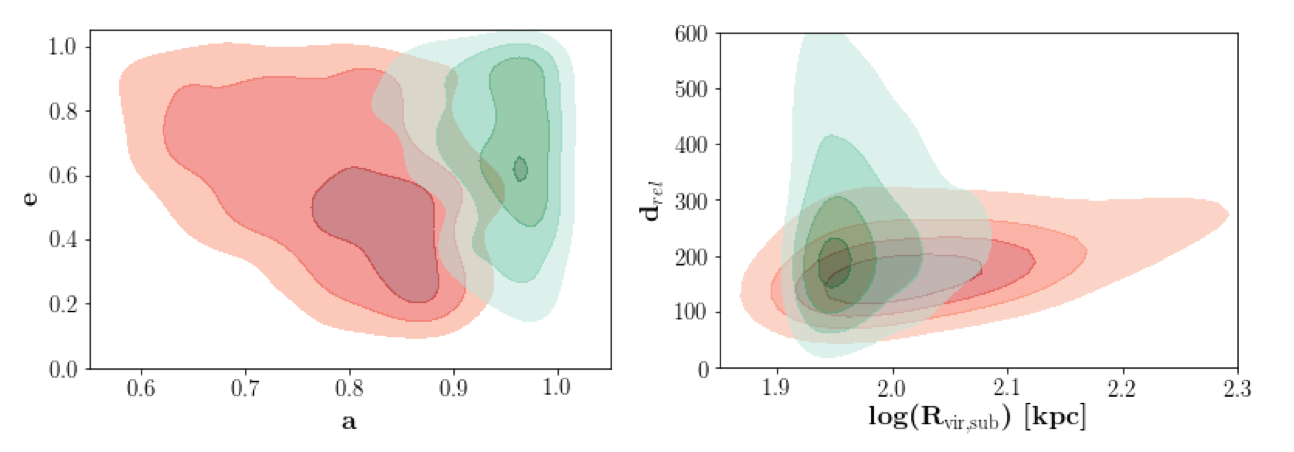
\includegraphics[width=\columnwidth]{Figures/massloss_contours}
	\vspace{-20pt}
    \caption{Contours of the top and bottom 25\% accuracies of predicted subhalos, in the two-dimensional spaces of the four most important features. Blue contours show the best predicted subhalos, and red contours show the worst predicted subhalos. Contours are divided into 5 sections, with 20\% of subhalos lying within the inner most contour, 40\% lying within the second innermost contour, and so on. The outermost contour is not shaded as to more clearly show the contour regions.}
    \label{fig:massloss_contours}
\end{figure}

Figure \ref{fig:massloss_predictions} shows the accuracy of best-fit model, when trained using all and increasingly small subsets of the feature parameters. Because accuracy of this model depends on the selected tolerance value, we show the accuracy given several different choices of tolerance. Again, the training set generally does better than the test set, for all tolerances, due to slight  overfitting. It can be seen that, using only the three top-ranking parameters, 60\% of subhalos have their final masses accurately predicted to with a margin of error of less than \textpm 5\% of their true initial mass. 90\% of subhalos can be predicted accurately, given predictions within \textpm 20\% of their initial mass. Almost all subhalos can have their masses predicted to within \textpm 50\% of their initial mass, although it's worth noting that, in the instance of a subhalo that loses half of its mass, that would allow the full range of losing none to all of its mass to be considered accurate. 

Although a significant fraction of our subhalo population cannot have their final masses predicted with high precision, we point out that this model still performs much better than a naive guess. As a baseline model, we assign a predicted final mass fraction to all subhalos as the average final mass fraction of the sample. Using Equation \ref{eq:mass loss} to calculate the accuracy of this baseline model, we find that only 15\% of subhalos have their final masses accurately predicted to with a margin of error of less than \textpm 5\% of their true initial mass, 65\% with a margin of error less than \textpm 20\% of their true initial mass, and 93\% with a margin of error less than \textpm 50\% of their true initial mass. It is clear that, although the majority of subhalos can be predicted to within \textpm 50\% of their true initial mass by both models, our machine learning model has much improvement over the baseline model for making more precise predictions.

The three parameters needed before prediction accuracy levels off with the addition of more parameters are: the radius of the subhalo, the initial scale factor, and the subhalo's orbital inclination. Again, given the ordering from the feature selection methods discussed above, these parameters show the quickest gain of information with the quickest leveling off of additional accuracy, even given a model allowed to select any of the full 26 parameter set. Adding these first three parameters results in an increase of \edits{\textbf{INSERT NUMBER}}, \edits{\textbf{INSERT NUMBER}}, and  \edits{\textbf{INSERT NUMBER}} accuracy percentage gain, respectively. We note that, because the radius and mass of subhalos are directly analytically related to one another, the radius can be replaced with the mass in this model with no difference in the information gain or final accuracy.

Within the parameter spaces of the four top parameters, we show in Figure \ref{fig:massloss_contours} where the subhalos with the best and worst 10\% of accuracy scores lie. Most of the best-predicted subhalos are those that enter their host closer to z=0, with the contours centering around a\textsubscript{i} = .95, likely because those do not have much time to lose mass before the end of the simulation, and thus have final masses similar to their initial masses. Larger subhalos, given by larger radii, also appear more difficult to predict than their smaller counterparts, with the span of radii for the best predicted subhalos being both centered around smaller radii and not spanning to large radii. As the radius of a subhalo is analog to its mass, this also means that less massive subhalos are easier to predict than their more massive counterparts. The best predicted subhalos also seem to have higher eccentricities than their poorly predicted counterparts, although the span of eccentricities is the same for both. The span of initial relative distances is different for the best and worst predicted populations, with the best predicted subhalos spanning across a larger range of relative distances, despite the centers of the contours being roughly the same.

We again want to determine if there are significant differences between the best and worst predicted subhalos with respect to our additional parameters. We perform a KS test between these distributions, with respect to each of the additional parameters beyond our set of the most important four, after finding a narrow bin within these four parameters that removes all differences between the best and worst predicted halos with respect to those four parameters. The KS test again shows that the two distributions have a detection above 3\textsigma to be the same, for all of our additional parameters, meaning that all of our additional parameters have no trend with the goodness of our predictions.

\subsection{Final Position}
\label{sec:position}
For only subhalos that survive until z=0 without being disrupted, we next predict the final position of the subhalo at z=0, relative to the center of the host halo, using a gradient boosting regressor. We tune the hyperparameters of this model and find the best results given 1800 estimators, a learning rate of .008, and a \textit{max\_depth} of 6. We keep the \textit{max\_leaf\_nodes} hyperparameter set to the default (None), allowing an unlimited number of nodes at each depth. To determine the accuracy of the model, we define an accuracy metric, using the the difference between true and predicted fractional distance from host center. A subhalo is considered to be accurately predicted if:
\begin{equation}
    \label{eq:position}
    |d_\textsubscript{rel,f,true} - d_\textsubscript{rel,f,pred}| - \frac{2R\textsubscript{soft}}{R_\textsubscript{host,f}} \leq tol
\end{equation}
Where \textit{tol} is some tolerance value which determines what difference in fractional distance from host center is acceptable as accurate. As when predicting the mass loss quantity, the left hand side of this equation determines the accuracy score, and we vary the tolerance to set different thresholds for what accuracy score we will consider as an accurate prediction. The first term in this equation is simply the absolute difference between the true and predicted fractional distance from host center. Because what our model predicts is the actual fractional distance of the subhalo from the host halo center, we do not need to additionally normalize this quantity as we did when predicting mass loss, as this value can be straightforwardly taken as the fraction of the host radius by which the prediction is off. The second term in the equation is an additional tolerance, to account for uncertainty in the subhalo's position within its host due to the softening length.

Figure \ref{fig:position_predictions} shows the accuracy of best-fit model, when trained using all and increasingly small subsets of the feature parameters. Because accuracy of this model depends on the selected tolerance value, we show the accuracy given several different choices of tolerance. Again, the training set generally does better than the test set, for all tolerances, due to slight  overfitting. For final position, it appears that more parameters are needed to reach maximum accuracy, with the first five given parameters being used for predictions before accuracy levels off. For final position, predictions are slightly worse than for mass loss. 50\% of subhalos can be predicted to \textpm 5\% of their true fractional distance. 90\% of subhalos can be predicted accurately, given their prediction requires accuracy to only \textpm 20\% of their true fractional distance. Almost all subhalos can have their final position predicted to within \textpm 50\% of their final fractional mass. As with mass loss, we note that a tolerance of .5 is very lenient, allowing the full range of the subhalo lying anywhere within the host as an accurate prediction.

We again compare the accuracy of these predictions to a baseline model, where we assign the average fractional distance from the host center of all subhalos to every subhalo in the sample. Using Equation \ref{eq:position} to calculate the accuracy of this baseline model, we find that 13\% of subhalos are correctly predicted when using a tolerance of .05, 47\% of subhalos are correctly predicted given a tolerance of .2, and 99\% of subhalos are correctly predicted using a tolerance of .5. Given that the average final fractional distance for subhalos is around .55, the 99\% correct predictions is unsurprising, as it means that  almost all subhalos with final positions within their hosts (which is all of them) are considered correctly predicted. Comparing these baseline accuracies at the .05 and .2 tolerance levels shows us that, although our machine learning model is only able to make precise position predictions for around half of our sample, this is a significant improvement over a simpler model.

The five parameters needed before prediction accuracy levels off with the addition of more parameters are: the radius of the host halo, the initial scale factor, the mass ratio between the sub and host halo, the subhalo's orbital inclination, and the relative velocity with which the subhalo enters. Given the ordering from the feature selection methods discussed above, it appears that these parameters were chosen to be quite important, although the mass ratio provides less accuracy gain than some of the other, later-chosen parameters. Adding these first five parameters results in an increase of \edits{\textbf{INSERT NUMBER}}, \edits{\textbf{INSERT NUMBER}}, \edits{\textbf{INSERT NUMBER}}, \edits{\textbf{INSERT NUMBER}}, and  \edits{\textbf{INSERT NUMBER}} accuracy percentage gain, respectively. Within the parameter spaces of the four top parameters, we show in Figure \ref{fig:position_contours} where the best and worst 10\% of predicted subhalos lie. Most of the best-predicted subhalos are those that enter their host closer to z=0, likely because those have less time to move deep into the host and have their orbits altered as much. The radius of the host appears to span roughly the same space for both populations, with the worst predicted subhalos being concentrated more towards smaller host radii than their better predicted counterparts. The two-dimensional space of mass ratio and orbital inclination is nearly identical for the two populations.

We again check the distributions of the best and worst predicted subhalos with respect to each of our additional parameters, beyond our set of the most important four. After controlling for a, \texttheta, and mass ratio by selecting a narrow bin in this parameter space where the two distributions of best and worst predicted suhalos are the same, we perform a KS test between the two distributions with respect to all additional parameters. In doing so, we find that the two distributions are the same, with a detection above 3\textsigma, except for the concentration of the subhalo and the eccentricity.

\begin{figure}
	% To include a figure from a file named example.*
	% Allowable file formats are eps or ps if compiling using latex
	% or pdf, png, jpg if compiling using pdflatex
	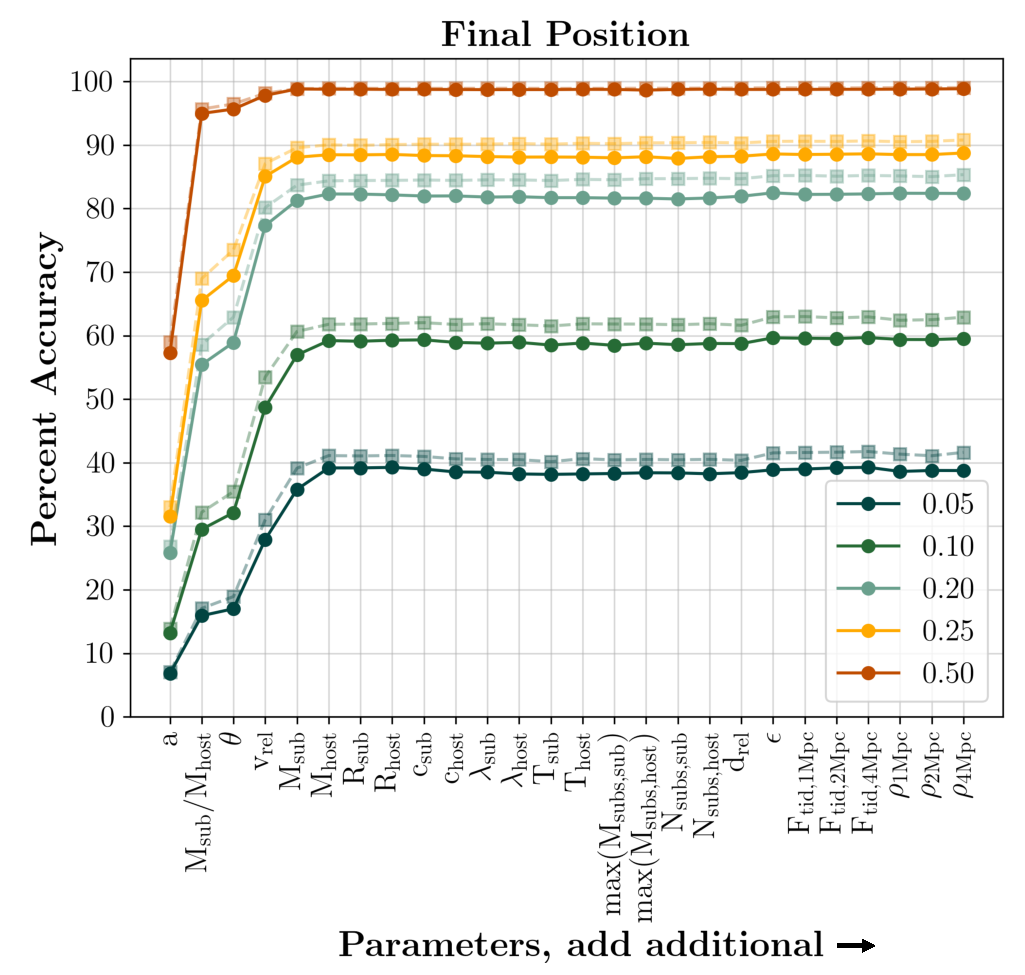
\includegraphics[width=\columnwidth]{Figures/position_predictions}
	\vspace{-15pt}
    \caption{Same as Figure \ref{fig:massloss_predictions}, but for the final position prediction. Different colored lines show the different tolerance values used to define accuracy, as defined in Equation \ref{eq:position}. For a complete description of this accuracy metric, see text.}
    \label{fig:position_predictions}
\end{figure}

\begin{figure}
	% To include a figure from a file named example.*
	% Allowable file formats are eps or ps if compiling using latex
	% or pdf, png, jpg if compiling using pdflatex
	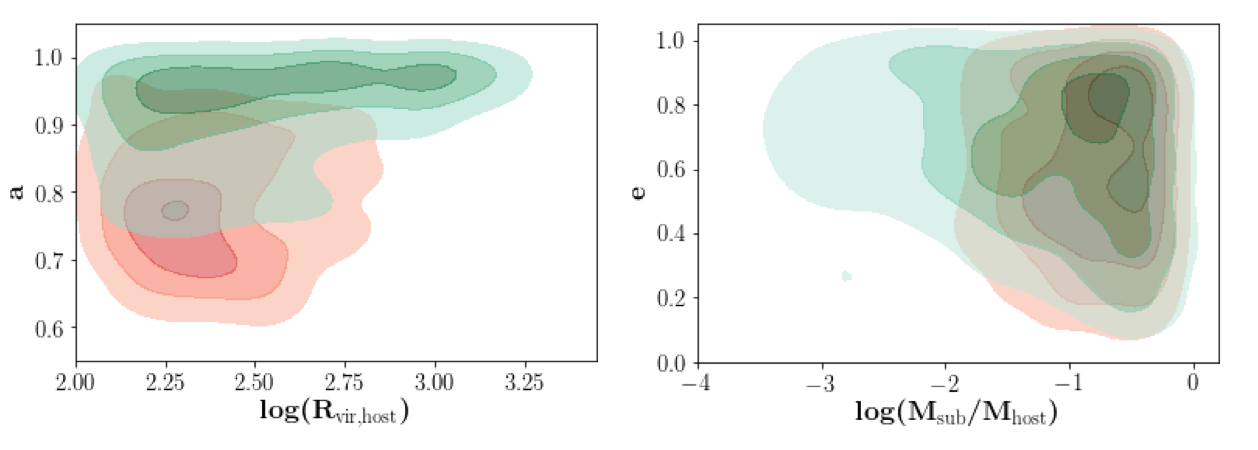
\includegraphics[width=\columnwidth]{Figures/position_contours}
	\vspace{-20pt}
    \caption{Same as \ref{fig:massloss_contours}, but for the final position parameters and predictions.}
    \label{fig:position_contours}
\end{figure}

\subsection{Merge Time}
\label{sec:merge time}
For only subhalos that have merged before z=0, we predict the amount of elapsed time between the subhalos entry and subsequent merging, using a gradient boosting regressor. We tune the hyperparameters of this model and find the best results given 500 estimators, a learning rate of .05, and a \textit{max\_depth} of 5. We keep the \textit{max\_leaf\_nodes} hyperparameter set to the default (None), allowing an unlimited number of nodes at each depth. To determine the accuracy of the model, we define an accuracy metric, using the the difference between true and predicted number of crossing times. A subhalo is considered to be accurately predicted if:
\begin{equation}
    \label{eq:time}
    \frac{|t_\textsubscript{f,true} - t_\textsubscript{f,pred}|}{t_\textsubscript{cross,f,true}} \leq tol
\end{equation}
Where \textit{tol} is some tolerance value which determines to within how many crossing times a prediction is considered to be accurate. As with our other final quantities, the left hand side of this equation determines the accuracy score, and we vary the tolerance to set different thresholds for what accuracy score we will consider as an accurate prediction. This accuracy score is calculated as the difference between the true and predicted elapsed time of infall for the subhalo, normalized by its final crossing time. Normalizing by this crossing time allows us to use this accuracy metric for all subhalos, regardless of when the merging interaction occurs.

Figure \ref{fig:time_predictions} shows the accuracy of best-fit model, when trained using all and increasingly small subsets of the feature parameters. Because accuracy of this model depends on the selected tolerance value, we show the accuracy given several different choices of tolerance. Again, the training set generally does better than the test set, for all tolerances, due to slight  overfitting. To predict merging time, again only three parameters appear to be necessary to reach maximum accuracy. 50\% of subhalos can be predicted to within half of a crossing time. 90\% of subhalos can be predicted accurately, given their prediction requires accuracy to only within 1.5 crossing times. All subhalos can have their merging time predicted to within five crossing times. Again, we emphasize that 5 crossing times is typically around 1 billion years.

As a baseline model to compare these results to, we assign to each subhalo the average number of crossing times of all subhalos to merge. Then, we use Equation \ref{eq:time} to check the accuracy of this simple model and compare it to the accuracy of our machine learning model. We find that, using this baseline model, \edits{\textbf{INSERT NUMBER}\%} of subhalos are correctly predicted to within .5 crossing times, \edits{\textbf{INSERT NUMBER}\%} of subhalos are correctly predicted to within 1.5 crossing times, and \edits{\textbf{INSERT NUMBER}\%} of subhalos are correctly predicted to within 5 crossing times. Again, although our model does not consistently make precise predictions, when comparing to a simpler baseline model, it performs significantly better.

The three parameters needed before prediction accuracy levels off with the addition of more parameters are: the initial scale factor, the subhalos orbital inclination, and the mass ratio between the sub and host halo. Adding these first three parameters results in an increase of \edits{\textbf{INSERT NUMBER}}, \edits{\textbf{INSERT NUMBER}}, and  \edits{\textbf{INSERT NUMBER}} accuracy percentage gain, respectively. Within the parameter spaces of the four top parameters, we show in Figure \ref{fig:position_contours} where the best and worst 10\% of predicted subhalos lie. Most of the best predicted subhalos have masses slightly more similar to their host halos than their worst predicted counterparts. They also appear to enter their hosts at somewhat earlier times. The worst predicted subhalos also appear to be concentrated around lower concentrations than their better-predicted counterparts, although the complete span of concentrations is similar for both. The orbital inclination does not appear to be significantly different between the two populations.

We again check the distributions of the best and worst predicted subhalos with respect to each of our additional parameters, beyond our set of the most important four. After controlling for a, \texttheta, and mass ratio by selecting a narrow bin in this parameter space where the two distributions of best and worst predicted suhalos are the same, we perform a KS test between the two distributions with respect to all additional parameters. In doing so, we find that the two distributions are the same, with a detection above 3\textsigma, except for the concentration of the subhalo and the eccentricity.

\begin{figure}
	% To include a figure from a file named example.*
	% Allowable file formats are eps or ps if compiling using latex
	% or pdf, png, jpg if compiling using pdflatex
	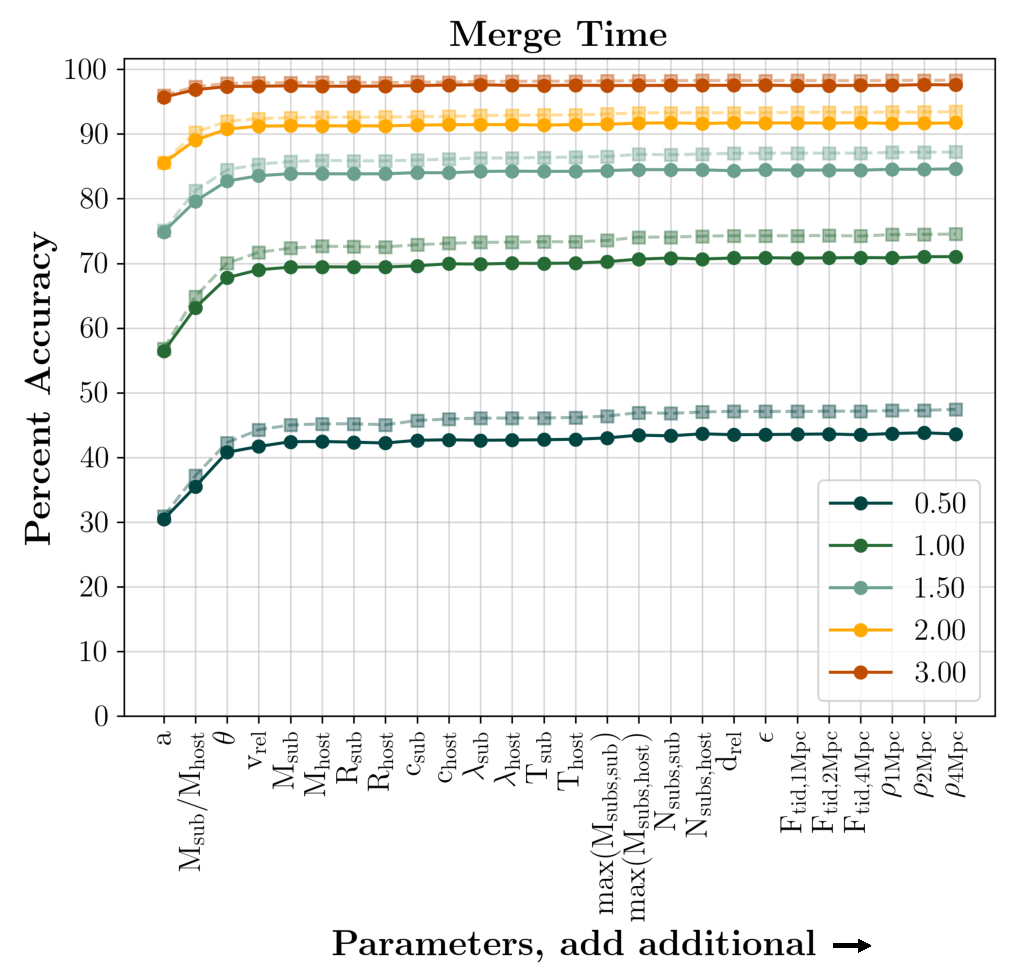
\includegraphics[width=\columnwidth]{Figures/time_predictions}
	\vspace{-15pt}
    \caption{Same as Figure \ref{fig:massloss_predictions}, but for the merge time prediction. Different colored lines show the different tolerance values used to define accuracy, as defined in Equation \ref{eq:time}. For a complete description of this accuracy metric, see text.}
    \label{fig:time_predictions}
\end{figure}

\begin{figure}
	% To include a figure from a file named example.*
	% Allowable file formats are eps or ps if compiling using latex
	% or pdf, png, jpg if compiling using pdflatex
	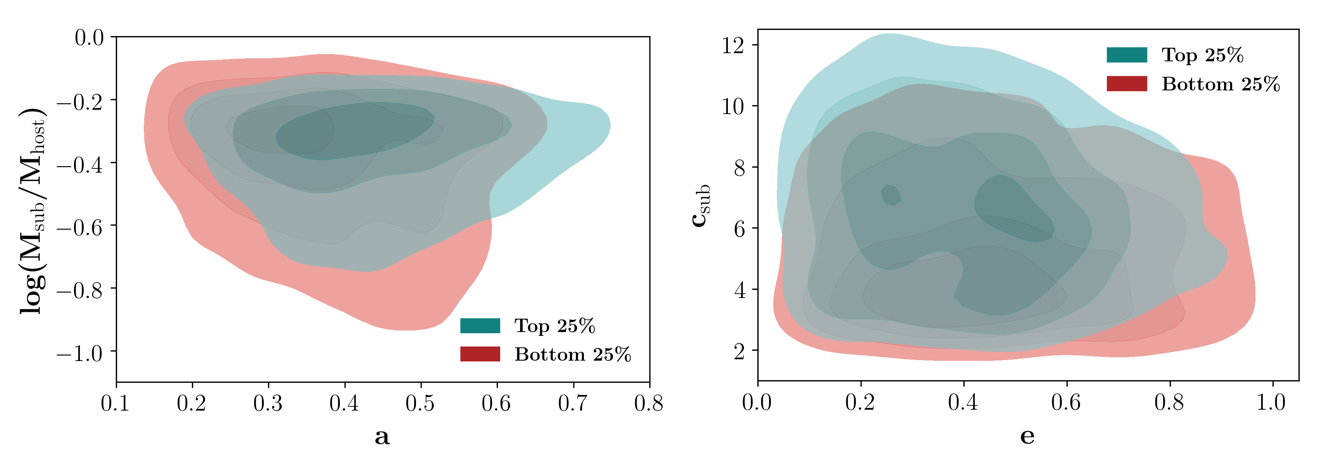
\includegraphics[width=\columnwidth]{Figures/time_contours}
    \vspace{-20pt}
    \caption{Same as \ref{fig:massloss_contours}, but for the merge time parameters and predictions.}
    \label{fig:time_contours}
\end{figure}


\section{Summary and Discussion}
\label{sec:Conclusion}
In this paper, we have used machine learning algorithms to fit models that predict the survival, mass loss, final position, and merge time of a subhalo from parameters taken right at the time of its infall. Our goal was to better understand to what degree these final outcomes are due to stochasticity in subhalo evolution versus real, physically-motivated processes that could be consistently, analytically predicted. From predictions based on these models, we have found:
\begin{itemize}
    \item Subhalo survival can be predicted remarkably well, with 96.5\% of our sample being correctly predicted as surviving or disrupting. These predictions need only three initial parameters: the scale factor at the time of the start of the interaction, the mass ratio between the subhalo and its host, and the orbital eccentricity. However, to reach this accuracy, the initial scale factor is by far the most influential of these parameters. Subhalos with both late and early entry times are easiest to predict, while those entering their host halos at a\textsubscript{i} = ~.65 are much more difficult. However, this is also dependent on the subhalo to host halo mass ratio, where subhalos with lower mass ratios instead having a region of uncertainty closer to  a\textsubscript{i} = \edits{\textbf{INSERT NUMBER}}.
    \item Subhalo mass loss is a generally stochastic process. Although for 60\% of our sample we were able to predict a final mass within \textpm5\% of the initial mass from the true final mass, we must loosen our criteria to \textpm20\% of the initial mass in order to consider 90\% of our sample correctly predicted. This maximum prediction accuracy is achieved using only three initial parameters: the radius of the subhalo, the scale factor at the time of the start of the interaction, and the orbital inclination. In general, our model makes better predictions for smaller subhalos with late entry times than for their larger or earlier counterparts.
    \item Subhalo final locations are also difficult to predict. 50\% of our sample can be correctly predicted to within \textpm5\% of their host radius, but an accuracy of 90\% is only achieved given predictions are accurate to within \textpm20\% of the host radius. These predictions need five initial parameters: the virial radius of the host halo, the scale factor at the time of the start of the interaction, the mass ratio between the sub and host halo, the orbital eccentricity, and the initial relative velocity. As with mass loss, our model makes better predictions for subhalos entering their hosts at later times. However, there does not seem to be a significant trend in prediction accuracy with regards to the other parameters that were found to be important for making these predictions. 
    \item Subhalo merging timescales are also difficult to predict. 50\% of our sample can be correctly predicted to within half of their initial crossing time, but an accuracy of 90\% is only achieved given predictions are accurate to within 1.5 crossing times. These predictions again need only three parameters: the scale factor at the time of the start of the interaction, the orbital eccentricity, and the mass ratio between the sub and host halo. 
    \item There are some interesting commonalities among both the sets of parameters needed to make these predictions and the parameter spaces in which predictions are poorest. Only five parameters, in total, are needed to achieve the maximum prediction accuracy for all of our predicted outcomes. The scale factor, orbital inclination, relative velocity, and the masses of the host and subhalo (sometimes combined as mass ratio or appearing as virial radius instead) appear to be the only relevant parameters for determining subhalo evolution. Additionally, the parameter spaces that are most difficult to make predictions within also have much overlap. In general, subhalos that enter at a mid-range of initial scales (typically a = .6-.8) are challenging to make predictions for, across all of our final outcomes. There also appear to be trends in inclination, with higher inclinations (more circular orbits) being easier to predict the behavior of, except for in the case of predicting disruption, where the opposite appears to be true.
    \item Additional parameters beyond the set needed to make predictions for each final quantity are not useful, either for making predictions or for generalizing the types of subhalos that are better or worse predicted. Although the best and worst predicted subhalos are typically distributed differently with respect to the parameters that are used to make predictions, when these parameters are controlled for, differences in these distributions with respect to all other parameters are removed. So, our additional parameters outside of the set used to make predictions do not correlate with the stochasticity of our predictions.
\end{itemize}

It is clear from our results that, for predicting the mass loss, final location, and merging timescales of individual subhalos, an accurate, consistent mapping cannot be found given our set of initial parameters. There are several possible reasons for this inability to accurately model subhalo evolution. The first possibility is that some parameter or parameters were missing from the initial set, which would have been fundamental to making accurate predictions. Although we have made sure to include an extensive list of physically-motivated parameters that were found in the literature to be important for modeling these outcomes, our list was not completely comprehensive with all possible information. For instance, Rockstar outputs \edits{\textbf{INSERT NUMBER 75?}} parameters about each subhalo, many of which encode information about the ID's of the halos, but also including: halfmass radius, largest shape ellipsoid axes, angular momenta, velocity dispersion, and some others, all which we decided not to include in our analysis here. However, we have no reason to believe that these excluded parameters would be able to contribute such a significant portion of the needed information as to make significant improvement to our predictions. So, although the possibility remains that additional parameters could be needed to improve predictions, it seems unlikely that the missing information could be completely encompassed there.

A second possibility is that errors within the simulation, halo catalog, or merger tree make subhalo evolution unpredictable and sometimes incorrect. Much speculation remains as to the accuracy of these simulations and their ability to accurately model the physics of subhalo evolution, particularly on these small scales (\citet{Kampen2005}, \citet{Taylor2005},\citet{VandenBosch2018}, \citet{Bosch2018}). Although several studies have suggested that simulation resolution only effects subhalos with small numbers of particles (\citet{Gao2004}, \citet{Nurmi2006}, \citet{Diemand2007}), \citet{VandenBosch2018} found that typical state-of-the-art cosmological simulations cannot resolve subhalos well enough to follow their mass loss until complete disruption. In the Bolshoi simulation, \citet{VandenBosch2017} found that only around 20\% of subhalo disruption was truly physical, with instantaneous masses of the subhalos along their orbits being highly erratic. Similarly, \citet{VandenBosch2018} found that most subhalo disruption in modern simulations is artificial or numerical in nature, with only subhalos in simulations of exquisite resolution (i.e softening lengths > .003 and greater than 10\textsuperscript{6} particles per halo) showing consistently converged results when orbiting close to the center of the host halo. A number of other works have also called into question the reliability of the halo catalogs and merger trees that are generated from these simulations. Comparison projects have found differing results for the fates of subhalos and the subhalo mass functions resulting from different halo finders (\citet{Knebe2011}, \citet{Onions2012}, \citet{Avila2014}, \citet{Bosch2014}, \citet{Behroozi2015}) and merger tree codes (\citet{Tweed2009}, \citet{Srisawat2013}, \citet{Jiang2014}). Because these codes fundamentally define subhalos in different ways and trace their properties between snapshots using different methods, these comparison projects found that, when applied to the same simulation, resulting halo catalogs and merger trees could differ quite significantly.

However, although the accuracy of simulation results have been brought into question, again, we note that it seems unlikely that these errors could be entirely responsible for the results we have found. \citet{Bosch2018} found that, despite physical disruption being extremely rare within simulations, subhalos only became highly sensitive to numerical disruption after losing over about 90\% of their mass. Additionally, even though \citet{Avila2014} found frequent fluctuations in the mass loss histories of subhalos within simulations using Rockstar, the overall mass losses were relatively smooth, and since our study only relies on final outcomes mapping from the initial conditions, minor errors along the history should not be important.

Another possibility is that final outcomes can be accurately predicted from initial conditions of the interaction, but the machine learning methods used here were not able to capture the process. This could be due to a few reasons. It is possible that the particular machine learning method used was not well-suited to the problem. However, we have extensively tried different algorithms, from very simple methods to neural networks, and have found that the results given here are the best we could possibly do. Another possibility is that we did not have enough data or the data did not span the space well enough. We also tested this by repeating our machine learning training and testing with smaller random subsets of our data, using instead one half and one quarter of our original sample, to ensure that our results did not change with fewer data points. In doing this, we found no change in maximum accuracy the model was able to reach, even with a significantly reduced amount of data.

The final possibility, and the one that we believe to be the most likely explanation, is that there is an inherent non-deterministic nature of these interactions. In this case, the initial conditions of an interaction are not enough to know the outcome, because similar initial conditions can lead to very different outcomes. This makes it impossible to train a model that relies on similar initial conditions producing similar outcomes to get consistent results. In Figure \ref{fig:stdev_bestSpaces}, we show the standard deviation of our final quantities within two-dimensional bins of the top two most important parameters for predicting them. It becomes clear in this figure that, even for very narrow ranges of parameter space, our outcomes can have a wide range of values. This further suggests that an inherent stochasticity within the merging process is likely the reason predictions are so difficult to get accurately. This also agrees with the contour plots shown in Figures \ref{fig:survival_contours}, \ref{fig:massloss_contours}, \ref{fig:position_contours}, and \ref{fig:time_contours}, which show that the regions of parameter space in which the machine learning models make the worst predictions are also the spaces in which there is the widest range of outcomes for similar initial conditions.

\begin{figure*}
	% To include a figure from a file named example.*
	% Allowable file formats are eps or ps if compiling using latex
	% or pdf, png, jpg if compiling using pdflatex
	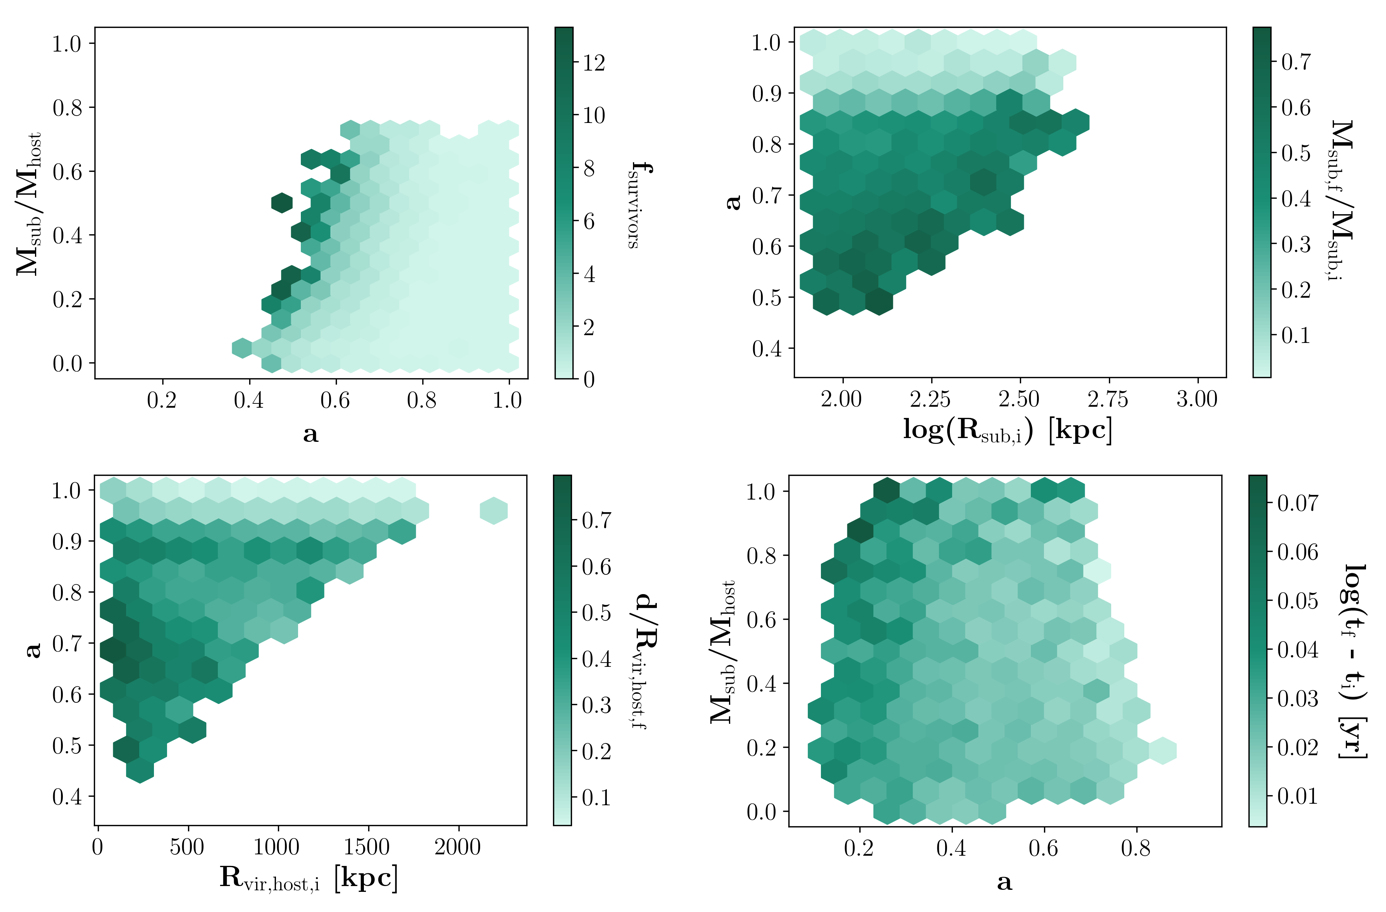
\includegraphics[width=\textwidth]{Figures/stdev_bestSpaces}
	\vspace{-20pt}
    \caption{Same as Figure \ref{fig:bestSpaces}, but each hexagonal bin contains the average standard deviation, normalized by the average value within that bin.}
    \label{fig:stdev_bestSpaces}
\end{figure*}

Several papers \citet{Angulo2009}, have noted that interactions between subhalos as they orbit within their hosts can be frequent and lead to significant amounts of mass loss. \citet{Tormen1998} found that penetrating interactions between subhalos can be the cause of nearly 40\% of a subhalos mass loss, whereas \citet{Knebe2005} found that the buildup of minor interactions over a subhalos life can be significant. \citet{Klimentowski2010} look at interactions between subhalos before they fall into their hosts, but find relatively weak interactions between halos in groups. \citet{Angulo2009} study the number of mergers between subhalos during their infall, and find that only a very small number of significant mergers occur. In our sample, we find that close interactions between our subhalos are quite common. A significant portion of our sample, \edits{\textbf{INSERT NUMBER}} of our subhalos, or around \edits{\textbf{INSERT NUMBER \%}} of our total sample, spend at least one timestep during their infall into their host as a sub-subhalo. That is, they enter the radius of another subhalo within the host, to have two or greater levels of hierarchy above them, at some point after they have entered the host themselves. After becoming a sub-subhalo, we find that \edits{\textbf{INSERT NUMBER}} of these subhalos, or around \edits{\textbf{INSERT NUMBER \%}} of our total sample, remain as sub-subhalos until they merge or until z = 0.

In order to test if these close interactions could either be a possible cause of the stochasticity that we've found or a deterministic effect that would better inform our predictions, we keep track of three additional parameters for each of our subhalos. The first is a flag that indicates whether, at any point during the infall, the subhalo becomes a sub-subhalo. The second is a flag that indicates whether the subhalo remains a sub-subhalo until either merging or z=0. The final extra parameter is the time that the subhalo spends being a sub-subhalo, totaled over all timesteps during which it in inside another subhalo. Since the subhalo can enter and then exit another subhalo multiple times, this number may reflect time spent inside more than one subhalo. In order to determine if any of these parameters hold predictive power, we try using them as extra parameters to each of our machine learning models. We find that, for all of our models, none of these parameters increase accuracy when added, meaning that the number and duration of interactions does not inform the evolution of our subhalo final quantities. We then try to determine if these interaction parameters could add stochasticity to the merging process and be responsible for the difficulty in making these predictions. We do this by using the same process we used to check if our other parameters added stochasticity, by checking if the distributions of the best and worst predicted subhalos are significantly different. For each model, we control for the parameters that were found to be important by selecting a narrow bin within each of them, then we perform a KS test between the distributions of best and worst predicted subhalos with respect to our interaction parameters. In doing so, we find that the two distributions are the same, with a detection above 3\textsigma, for all of our models. This suggests that these close interactions between subhalos are not important for their evolution as they fall into their hosts, neither by affecting the outcome nor by adding noise to the process.

\edits{Possible use/implications for simulation.}An inherent stochasticity in these merging processes within has implications for simulations and the models that are built from them.  \edits{What can we say about the results of simulations or how they do their calculations of these types of merging interactions based on the uncertainty in the outcomes of the objects? How much can we expect this type of uncertainty and is it a cause for concern.
 Can you still use these models to make predictions for galaxy evolution? Assigning populations from these distributions.}

\edits{Possible use/implications for observation. Is there anything we can say about distributions that we can expect around the MW or other galaxies. Particularly for survival which we obviously predict much better than the other quantities.} Although the inability to accurately model subhalo evolution points to stochasticity in merging processes, 

In this study, we have used a dark matter only simulation to study the evolution of subhalos. However, hydrodynamic simulations can also be used to study subhalo evolution, in the more complete context of baryonic physics as well. Several recent studies have found that the the presence of baryons can significantly effect the subhalos in which the galaxies reside (\citet{Dolag2009}, \citet{Romano-Diaz2010}, \citet{Brooks2013}, \citet{Sawala2016}, \citet{Garrison-Kimmel2017}). It remains to be seen and would be interesting to explore the implications of baryons in this type of work. Although subhalo disruption and evolution in dark matter only simulations appears stochastic and difficult to predict, hydrodynamic simulations may be differently behaved. Additionally, given that this type of work gives some insight as to what parameters are most prominent in determining how a subhalo evolves, a similar study using a hydrodyanmic simulation could confirm or oppose these findings, providing interesting insights to the differences between these types of simulations. 

\section*{Acknowledgements}

I would like to thank the academy, ...

%%%%%%%%%%%%%%%%%%%%%%%%%%%%%%%%%%%%%%%%%%%%%%%%%%

%%%%%%%%%%%%%%%%%%%% REFERENCES %%%%%%%%%%%%%%%%%%

% The best way to enter references is to use BibTeX:

\bibliographystyle{mnras}
\bibliography{mendeley.bib}

%%%%%%%%%%%%%%%%%%%%%%%%%%%%%%%%%%%%%%%%%%%%%%%%%%

%%%%%%%%%%%%%%%%% APPENDICES %%%%%%%%%%%%%%%%%%%%%

\appendix

\section{Some extra material}

If I wanted to present additional material which would interrupt the flow of the main paper, that would go here.

%%%%%%%%%%%%%%%%%%%%%%%%%%%%%%%%%%%%%%%%%%%%%%%%%%


% Don't change these lines
\bsp	% typesetting comment
\label{lastpage}
\end{document}

% End of mnras_template.tex